%package list
\documentclass{article}
\usepackage[top=3cm, bottom=3cm, outer=3cm, inner=3cm]{geometry}
\usepackage{multicol}
\usepackage{graphicx}
\usepackage{url}
%\usepackage{cite}
\usepackage{hyperref}
\usepackage{array}
%\usepackage{multicol}
\newcolumntype{x}[1]{>{\centering\arraybackslash\hspace{0pt}}p{#1}}
\usepackage{natbib}
\usepackage{pdfpages}
\usepackage{multirow}
\usepackage[normalem]{ulem}
\useunder{\uline}{\ul}{}
\usepackage{svg}
\usepackage{xcolor}
\usepackage{listings}
\lstdefinestyle{ascii-tree}{
    literate={├}{|}1 {─}{--}1 {└}{+}1 
  }
\lstset{basicstyle=\ttfamily,
  showstringspaces=false,
  commentstyle=\color{red},
  keywordstyle=\color{blue}
}
%\usepackage{booktabs}
\usepackage{caption}
\usepackage{subcaption}
\usepackage{float}
\usepackage{array}

\newcolumntype{M}[1]{>{\centering\arraybackslash}m{#1}}
\newcolumntype{N}{@{}m{0pt}@{}}


%%%%%%%%%%%%%%%%%%%%%%%%%%%%%%%%%%%%%%%%%%%%%%%%%%%%%%%%%%%%%%%%%%%%%%%%%%%%
%%%%%%%%%%%%%%%%%%%%%%%%%%%%%%%%%%%%%%%%%%%%%%%%%%%%%%%%%%%%%%%%%%%%%%%%%%%%
\newcommand{\itemStudent}{Arles Carrasco Choque, Jean Carlo Chara Condori, Reyser Zapata Butron, Daniela Choquecondo Aspilcueta}
\newcommand{\itemCourse}{Programación Web 2}
\newcommand{\itemCourseCode}{1702122}
\newcommand{\itemSemester}{III}
\newcommand{\itemUniversity}{Universidad Nacional de San Agustín de Arequipa}
\newcommand{\itemFaculty}{Facultad de Ingeniería de Producción y Servicios}
\newcommand{\itemDepartment}{Departamento Académico de Ingeniería de Sistemas e Informática}
\newcommand{\itemSchool}{Escuela Profesional de Ingeniería de Sistemas}
\newcommand{\itemAcademic}{2023 - A}
\newcommand{\itemInput}{Del 18 julio del 2023}
\newcommand{\itemOutput}{Al 26 julio del 2023}
\newcommand{\itemPracticeNumber}{08}
\newcommand{\itemTheme}{Django Rest Framework}
%%%%%%%%%%%%%%%%%%%%%%%%%%%%%%%%%%%%%%%%%%%%%%%%%%%%%%%%%%%%%%%%%%%%%%%%%%%%
%%%%%%%%%%%%%%%%%%%%%%%%%%%%%%%%%%%%%%%%%%%%%%%%%%%%%%%%%%%%%%%%%%%%%%%%%%%%

\usepackage[english,spanish]{babel}
\usepackage[utf8]{inputenc}
\AtBeginDocument{\selectlanguage{spanish}}
\renewcommand{\figurename}{Figura}
\renewcommand{\refname}{Referencias}
\renewcommand{\tablename}{Tabla} %esto no funciona cuando se usa babel
\AtBeginDocument{%
	\renewcommand\tablename{Tabla}
}

\usepackage{fancyhdr}
\pagestyle{fancy}
\fancyhf{}
\setlength{\headheight}{30pt}
\renewcommand{\headrulewidth}{1pt}
\renewcommand{\footrulewidth}{1pt}
\fancyhead[L]{\raisebox{-0.2\height}{
\includegraphics[width=3cm]{img/logo_episunsa.png}}}
\fancyhead[C]{\fontsize{7}{7}\selectfont	\itemUniversity \\ \itemFaculty \\ \itemDepartment \\ \itemSchool \\ \textbf{\itemCourse}}
\fancyhead[R]{\raisebox{-0.2\height}{
\includegraphics[width=1.2cm]{img/logo_abet}}}
\fancyfoot[L]{Grupo Laboratorio Pweb2}
\fancyfoot[C]{\itemCourse}
\fancyfoot[R]{Página \thepage}

% para el codigo fuente
\usepackage{listings}
\usepackage{color, colortbl}
\definecolor{dkgreen}{rgb}{0,0.6,0}
\definecolor{gray}{rgb}{0.5,0.5,0.5}
\definecolor{mauve}{rgb}{0.58,0,0.82}
\definecolor{codebackground}{rgb}{0.95, 0.95, 0.92}
\definecolor{tablebackground}{rgb}{0.8, 0, 0}

\lstset{frame=tb,
	language=bash,
	aboveskip=3mm,
	belowskip=3mm,
	showstringspaces=false,
	columns=flexible,
	basicstyle={\small\ttfamily},
	numbers=none,
	numberstyle=\tiny\color{gray},
	keywordstyle=\color{blue},
	commentstyle=\color{dkgreen},
	stringstyle=\color{mauve},
	breaklines=true,
	breakatwhitespace=true,
	tabsize=3,
	backgroundcolor= \color{codebackground},
}

\begin{document}
	
	\vspace*{10px}
	
	\begin{center}	
		\fontsize{17}{17} \textbf{ Informe de Laboratorio \itemPracticeNumber}
	\end{center}
	\centerline{\textbf{\Large Tema: \itemTheme}}
	%\vspace*{0.5cm}	

	\begin{flushright}
		\begin{tabular}{|M{2.5cm}|N|}
			\hline 
			\rowcolor{tablebackground}
			\color{white} \textbf{Nota}  \\
			\hline 
			     \\[30pt]
			\hline 			
		\end{tabular}
	\end{flushright}	

	\begin{table}[H]
		\begin{tabular}{|x{4.7cm}|x{4.8cm}|x{4.8cm}|}
			\hline 
			\rowcolor{tablebackground}
			\color{white} \textbf{Estudiante} & \color{white}\textbf{Escuela}  & \color{white}\textbf{Asignatura}   \\
			\hline 
			{\itemStudent} & \itemSchool & {\itemCourse \par Semestre: \itemSemester \par Código: \itemCourseCode}     \\
			\hline 			
		\end{tabular}
	\end{table}		
	
	\begin{table}[H]
		\begin{tabular}{|x{4.7cm}|x{4.8cm}|x{4.8cm}|}
			\hline 
			\rowcolor{tablebackground}
			\color{white}\textbf{Laboratorio} & \color{white}\textbf{Tema}  & \color{white}\textbf{Duración}   \\
			\hline 
			\itemPracticeNumber & \itemTheme & 04 horas   \\
			\hline 
		\end{tabular}
	\end{table}
	
	\begin{table}[H]
		\begin{tabular}{|x{4.7cm}|x{4.8cm}|x{4.8cm}|}
			\hline 
			\rowcolor{tablebackground}
			\color{white}\textbf{Semestre académico} & \color{white}\textbf{Fecha de inicio}  & \color{white}\textbf{Fecha de entrega}   \\
			\hline 
			\itemAcademic & \itemInput &  \itemOutput  \\
			\hline 
		\end{tabular}
	\end{table}
	
\section{Ejercicio}
	\begin{itemize}		
		\item Practique desarrollando el ejercicio de iniciación:
		\item \url{https://www.django-rest-framework.org/tutorial/quickstart/}
		\item Para consumir el web-service puede usar el cliente SOAP UI Community: \url{https://www.soapui.org/downloads/soapui/}
	\end{itemize}

        \textbf{Solución:}
        Después de seguir los pasos dados en la documentación de Django Rest Framework, se logra obtener una api gráfica que se puede acceder haciendo login como super usuario, obteniendo así la siguiente imagen en nuestra pantalla. \\
        
        Para poder ejecutar este proyecto, debemos seguir los siguientes comandos en nuestra terminal:

        \begin{lstlisting}[language=bash,caption={Ingresango a la carpeta Tutorial}][H]
		$ cd Tutorial
	\end{lstlisting}

        Ahora debemos abrir el servidor manage.py
        
        \begin{lstlisting}[language=bash,caption={Abriendo el servidor del ejercicio}][H]
		$ python .\manage runserver
	\end{lstlisting}

        Luego de hacer estos pasos, podemos ver el proyecto del ejercicio en ejecución
        
        \begin{figure}[H]
            \centering
            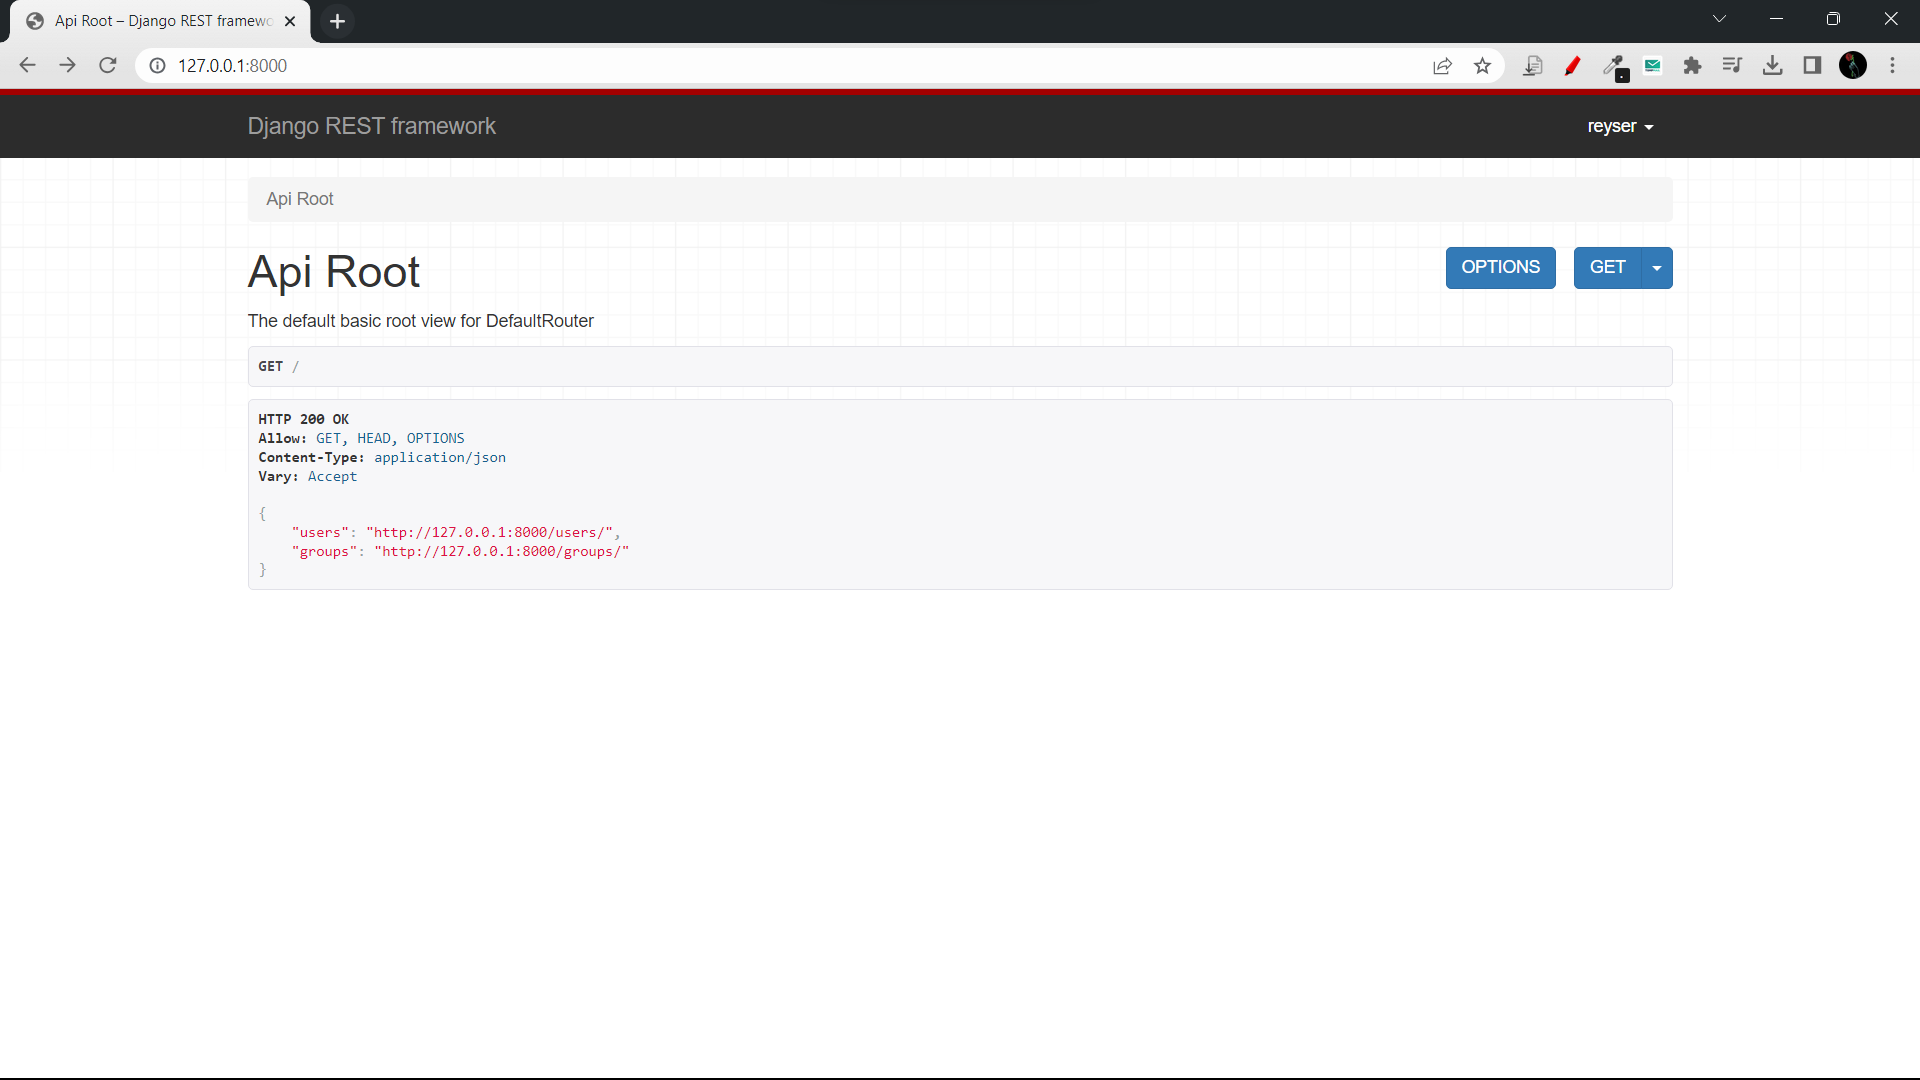
\includegraphics[width=0.9\textwidth,keepaspectratio]{img/ejercicioMain.png}
            \caption{Captura de pantalla del manage.py de tutorial}
            \label{fig:enter-label}
        \end{figure}
        
        Si accedemos a Users, nos devolverá los datos de la API, que en este caso serían todos los usuarios registrados en el panel admin de Django:
        
        \begin{figure}[H]
            \centering
            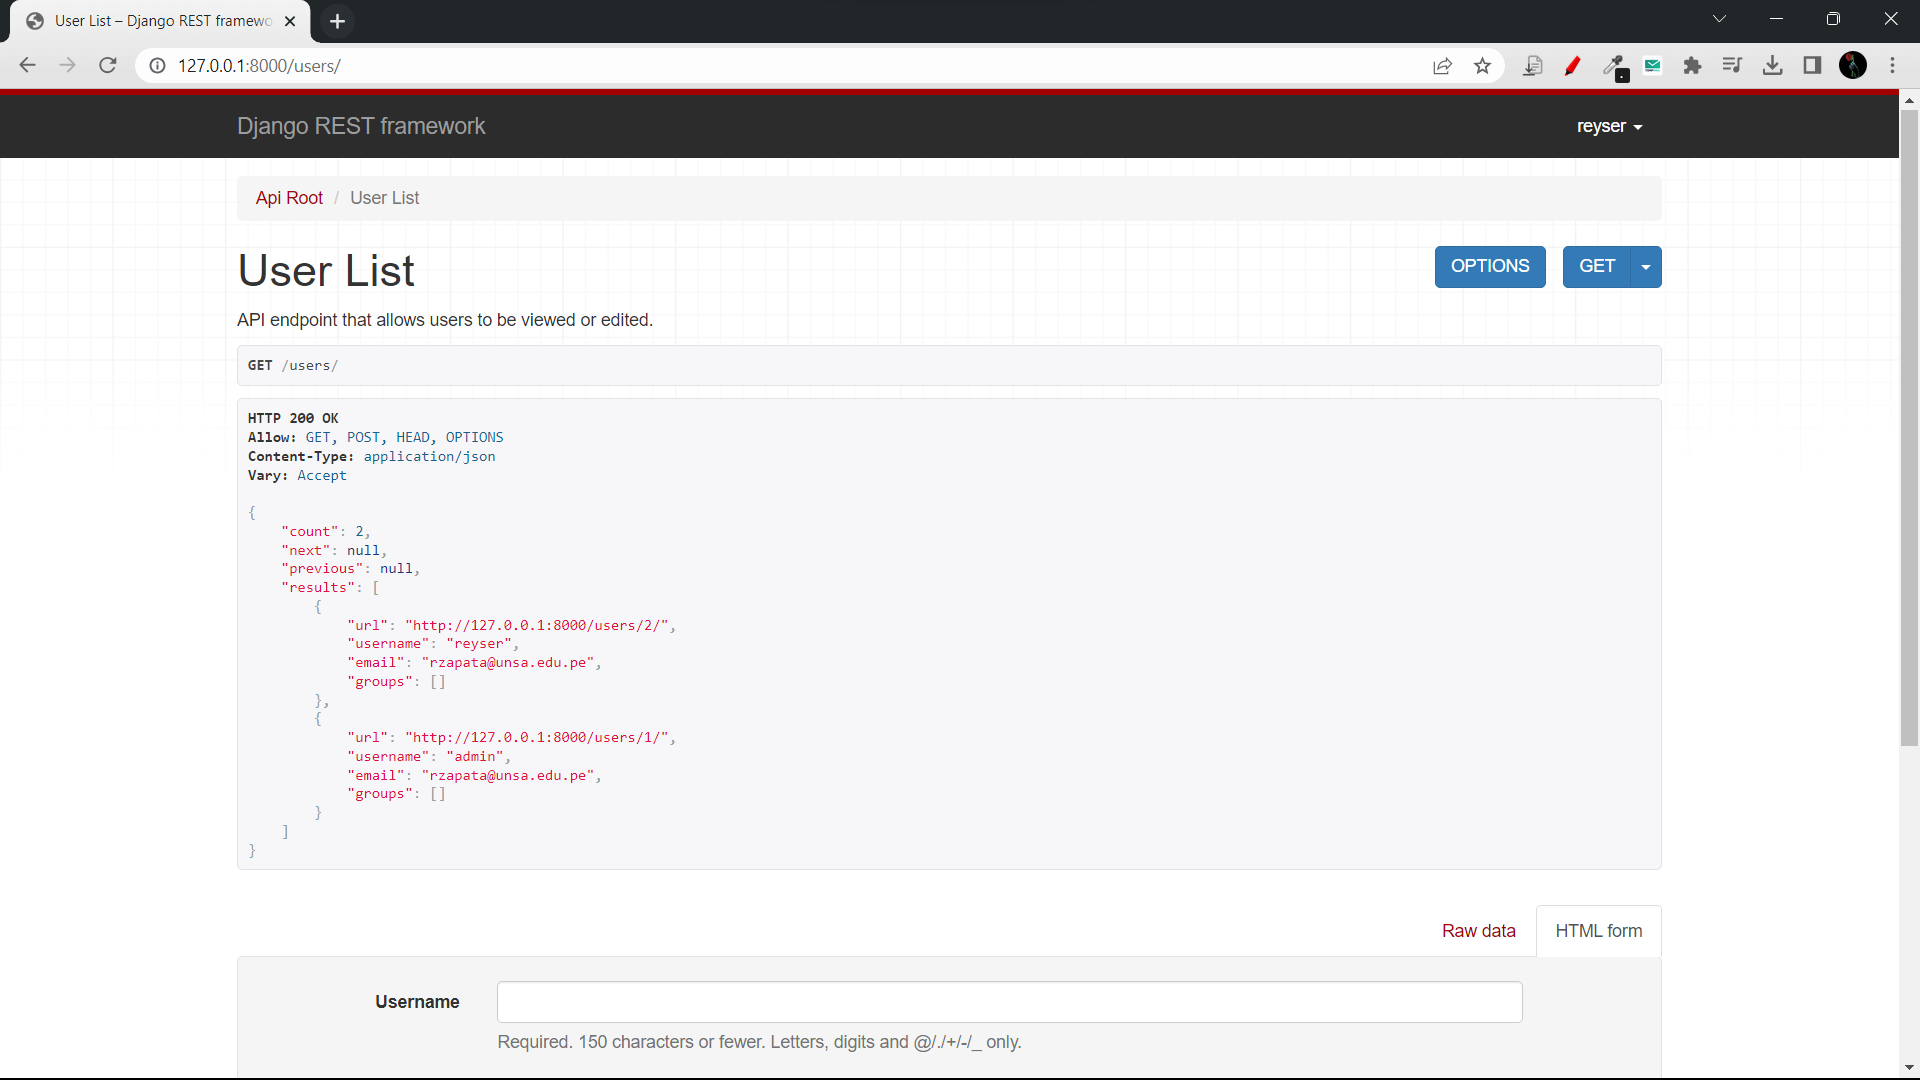
\includegraphics[width=0.9\textwidth,keepaspectratio]{img/ejercicio.png}
            \caption{Captura de pantalla de Users API}
            \label{fig:enter-label}
        \end{figure}

        Se logró una explicación eficiente y clara del funcionamiento de Django Rest Framework, un requisito esencial para la tarea asignada. Gracias a esta explicación, se pudo comprender a fondo cómo funcionan las APIs y cómo interactúan con la plataforma.

\section{Tarea}
\begin{itemize}
    \item En sus grupos de trabajo correspondientes. Elabore un servicio web que tenga un CRUD con el uso de este framework
    \item Create - POST
    \item Read - GET
    \item Update - PUT
    \item Delete - DELETE
    \item Centrarce en el Core business de su aplicacion web. Los mas importante y necesario que este disponible a traves de un servicio web.
    \item Ejemplos: \url{https://reqbin.com/}, \url{https://www.googleapis.com/youtube/v3/playlistItems}
    \item Muestre la funcionalidad consumiendola desde el cliente Rest de su preferencia.
    \item El metodo GET puede ser directamente consumido por un navegador web:
    \item Por ejemplo: En esta API se puede obtener la temperatura de Arequipa en un rango de fechas: (La version gratuita tiene un retraso de 7 días, por tanto solo mostrará la temperatura en Arequipa desde el 01 de Julio hasta el 03 de Julio)
    \item \url{https://archive-api.open-meteo.com/v1/archive?latitude=-16.39889&longitude=-71.535&amp}
\end{itemize}

\subsection{Crear una API con respuesta en JSON}
\textbf{Solución:} \\
Para completar todos los requerimientos de este laboratorio, se hizo 2 proyectos django, "DjangoApiRest" y "dniAPI", en el que podremos apreciar como funciona, una API y un servicio web consumiendo una API de validación. \\

Primero explicaremos el proyecto Principal que resuelve la tarea, "DjangoApiRest", es nuestra API de contactos. El Core Business de nuestra API de contactos sería gestionar y proporcionar acceso a la información relacionada con los contactos almacenados en nuestro sistema. Esto incluiría operaciones para listar todos los contactos, buscar un contacto específico por su ID, agregar nuevos contactos, actualizar la información de un contacto existente y eliminar contactos.\\

Ahora mostraremos los codigos de los archivos más relevantes de este proyecto y posteriormente de la app:

\subsubsection{Proyecto DjangoApiRest}

    \lstinputlisting[language=Python, caption={DjangoApiRest/urls.py},numbers=left,]{src/urls.py}

    Este es el Urls.py del proyecto, en el que definimos nuestra url principal, que sería "api/get/", para que así al abrir nuestro servidor, se nos muestre todos los contactos.

    \lstinputlisting[language=Python, caption={DjangoApiRest/middleware.py},numbers=left,]{src/middleware.py}

    Este archivo es un Middleware, con la clase JsonRespondeMiddleware, encargado de que todo lo que nos responda nuestro servidor, sea en formato JSON, así como se pide en la tarea

\subsubsection{App api}
En la app de nuestro proyecto, está lo escencial de que nuesta Api funcione y haga todo eficiente:

   \lstinputlisting[language=Python, caption={DjangoApiRest/urlsApi.py},numbers=left,]{src/urlsApi.py}

    En esta urls de nuestra app api, definimos las urls con las diferentes opciones de un CRUD (GET, POST, PUT, DELETE), cada uno teniendo una url y función diferente

    \lstinputlisting[language=Python, caption={DjangoApiRest/views.py},numbers=left,]{src/views.py}

    Este es el codigo que nos permitira recibir un request y devolver un JSON en pantalla, cada uno tiene su propia funcionalidad

    \lstinputlisting[language=Python, caption={DjangoApiRest/models.py},numbers=left,]{src/models.py}

    Este es el modelos de los Contactos, cada uno con su proposito

    \lstinputlisting[language=Python, caption={DjangoApiRest/serializers.py},numbers=left,]{src/serializers.py}

    Finalmente, el serializer que nos permitirá darle formato a nuestra API, convirtiendola en 100x100 API

    \subsubsection{Ejecución}
    Como es un API CRUD, tendremos que ver las diferentes acciones, con "Thunder Cliente" de Visual Studio Code, que nos permitira saber si nuestra api está recibiendo y devolviendo lo que deseamos y tambien consumirla desde el navegador web, demostrando su eficiencia.

    Primero debemos ejecutar el servidor, nuestro manage.py es el que está en el directorio principal.
    
    \begin{lstlisting}[language=bash,caption={Abriendo servidor}][H]
		$ python .\manage.py runserver
    \end{lstlisting}

    \textbf{GET} - 
    Este GET, es general, devuelve todos los contactos de la base de datos.
        \begin{figure}[H]
            \centering
            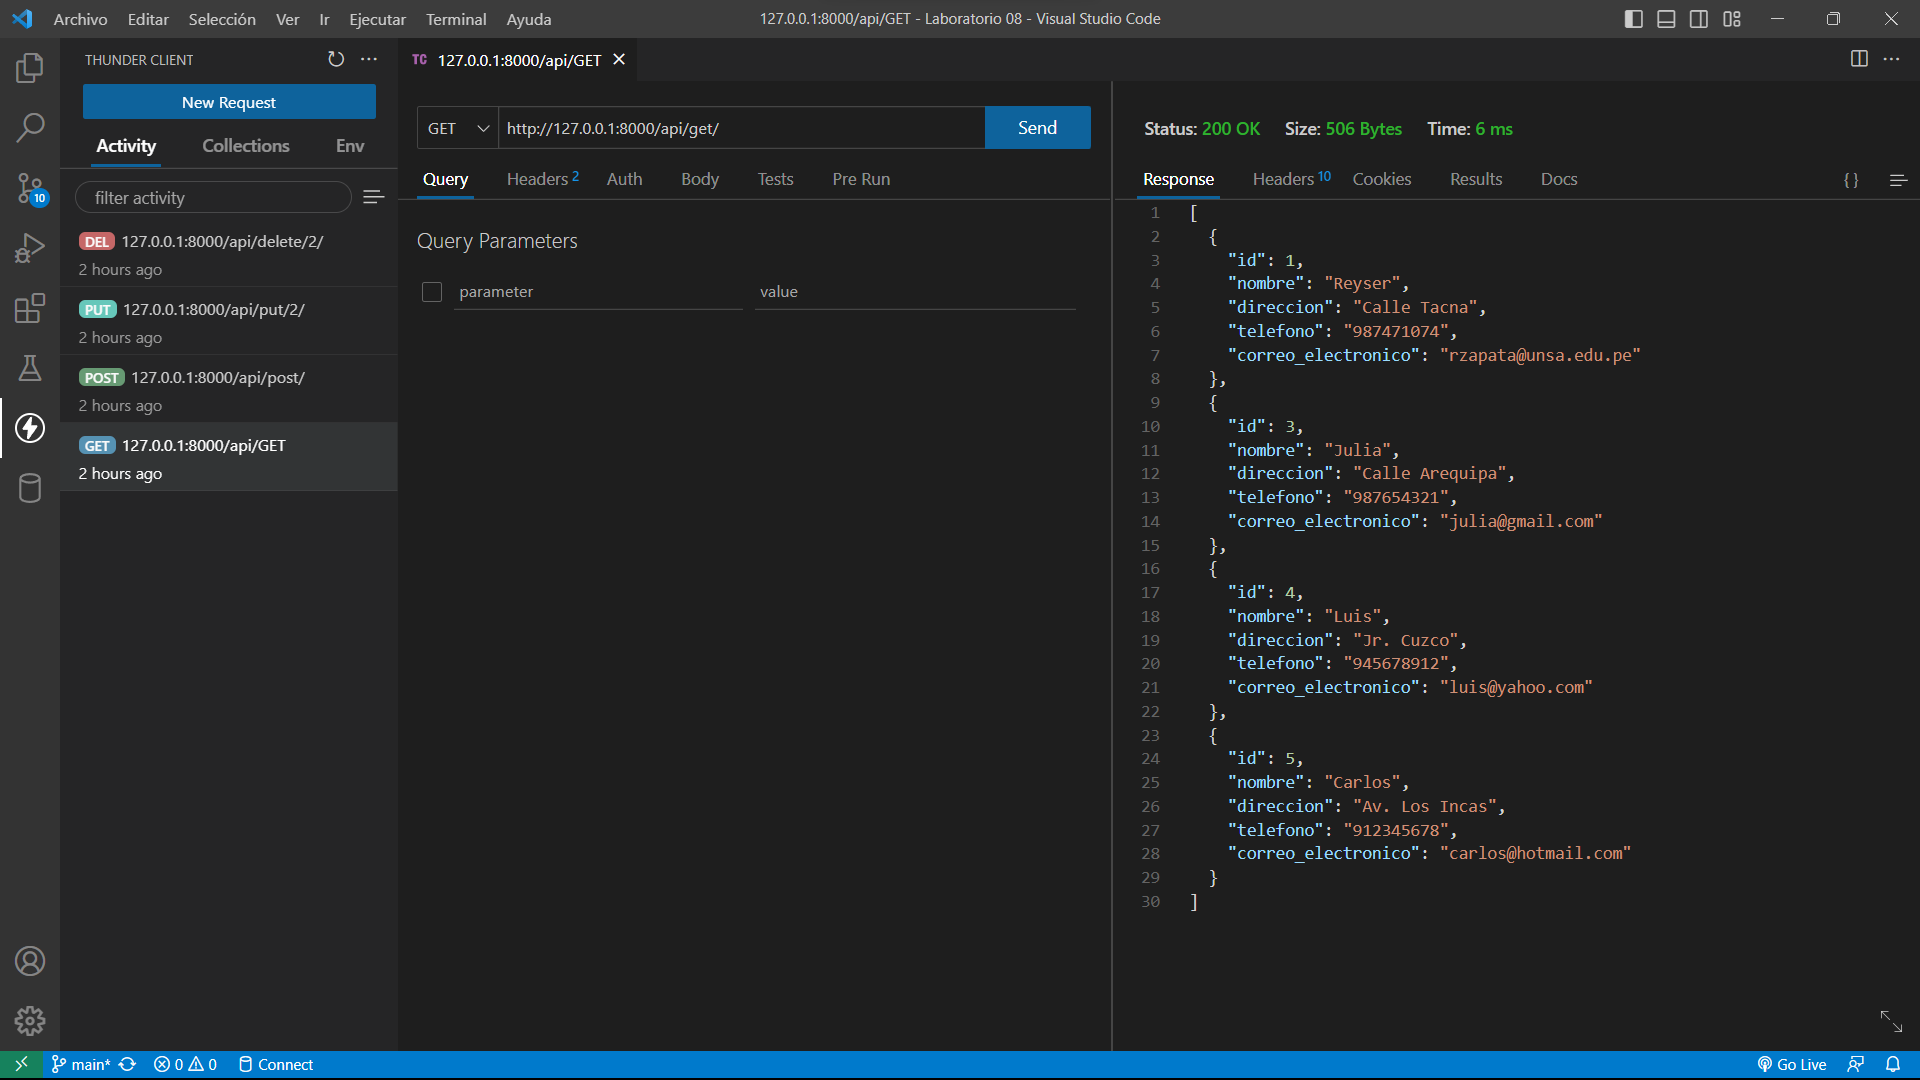
\includegraphics[width=0.9\textwidth,keepaspectratio]{img/DjangoApiRest/get1.png}
            \caption{GET de todos los Contactos desde Thunder Client}
            \label{fig:enter-label}
        \end{figure}

        \begin{figure}[H]
            \centering
            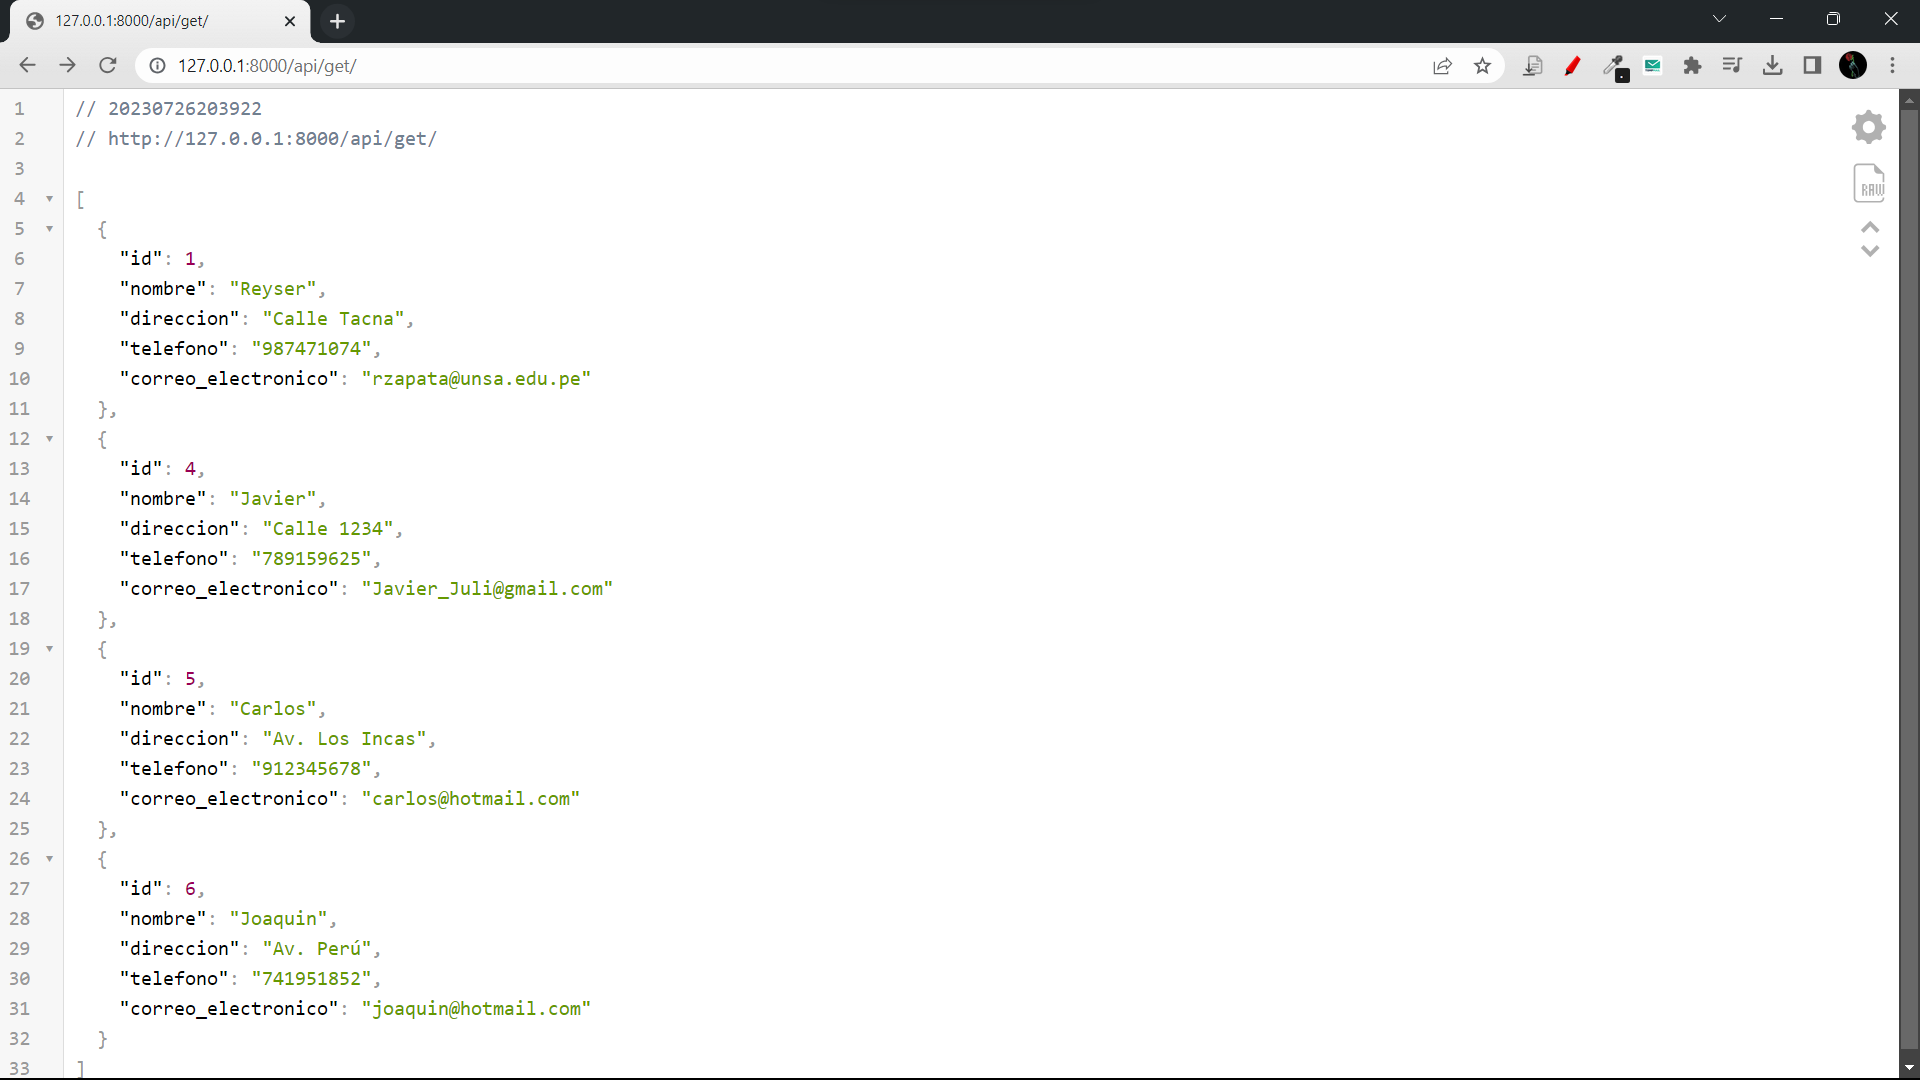
\includegraphics[width=0.9\textwidth,keepaspectratio]{img/DjangoApiRest/getWeb1.png}
            \caption{GET de todos los Contactos desde la web}
            \label{fig:enter-label}
        \end{figure}

    \textbf{GET/id/} - 
    Este GET, es especifico, devuelve solo 1 contacto de acuerdo al id ingresado en la url.
        \begin{figure}[H]
            \centering
            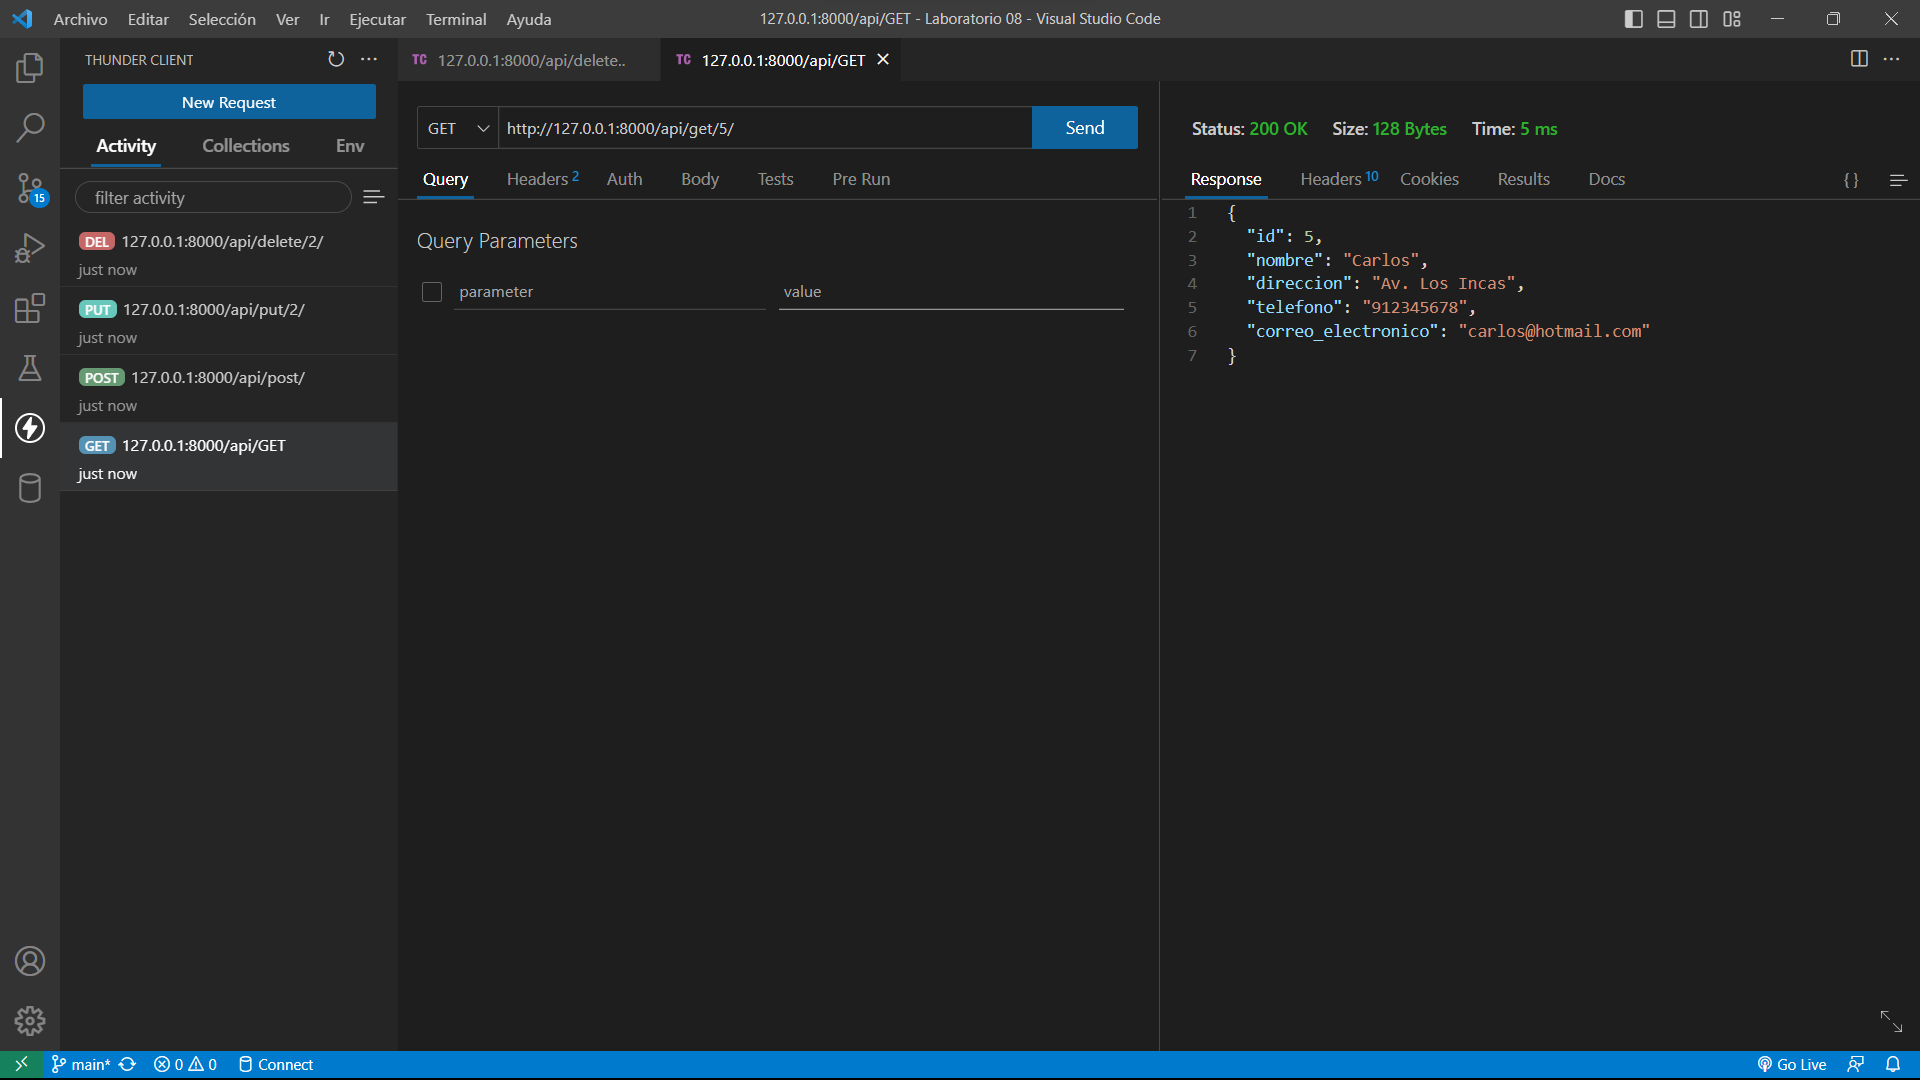
\includegraphics[width=0.9\textwidth,keepaspectratio]{img/DjangoApiRest/get2.png}
            \caption{GET de un contacto desde Thunder Client}
            \label{fig:enter-label}
        \end{figure}

        \begin{figure}[H]
            \centering
            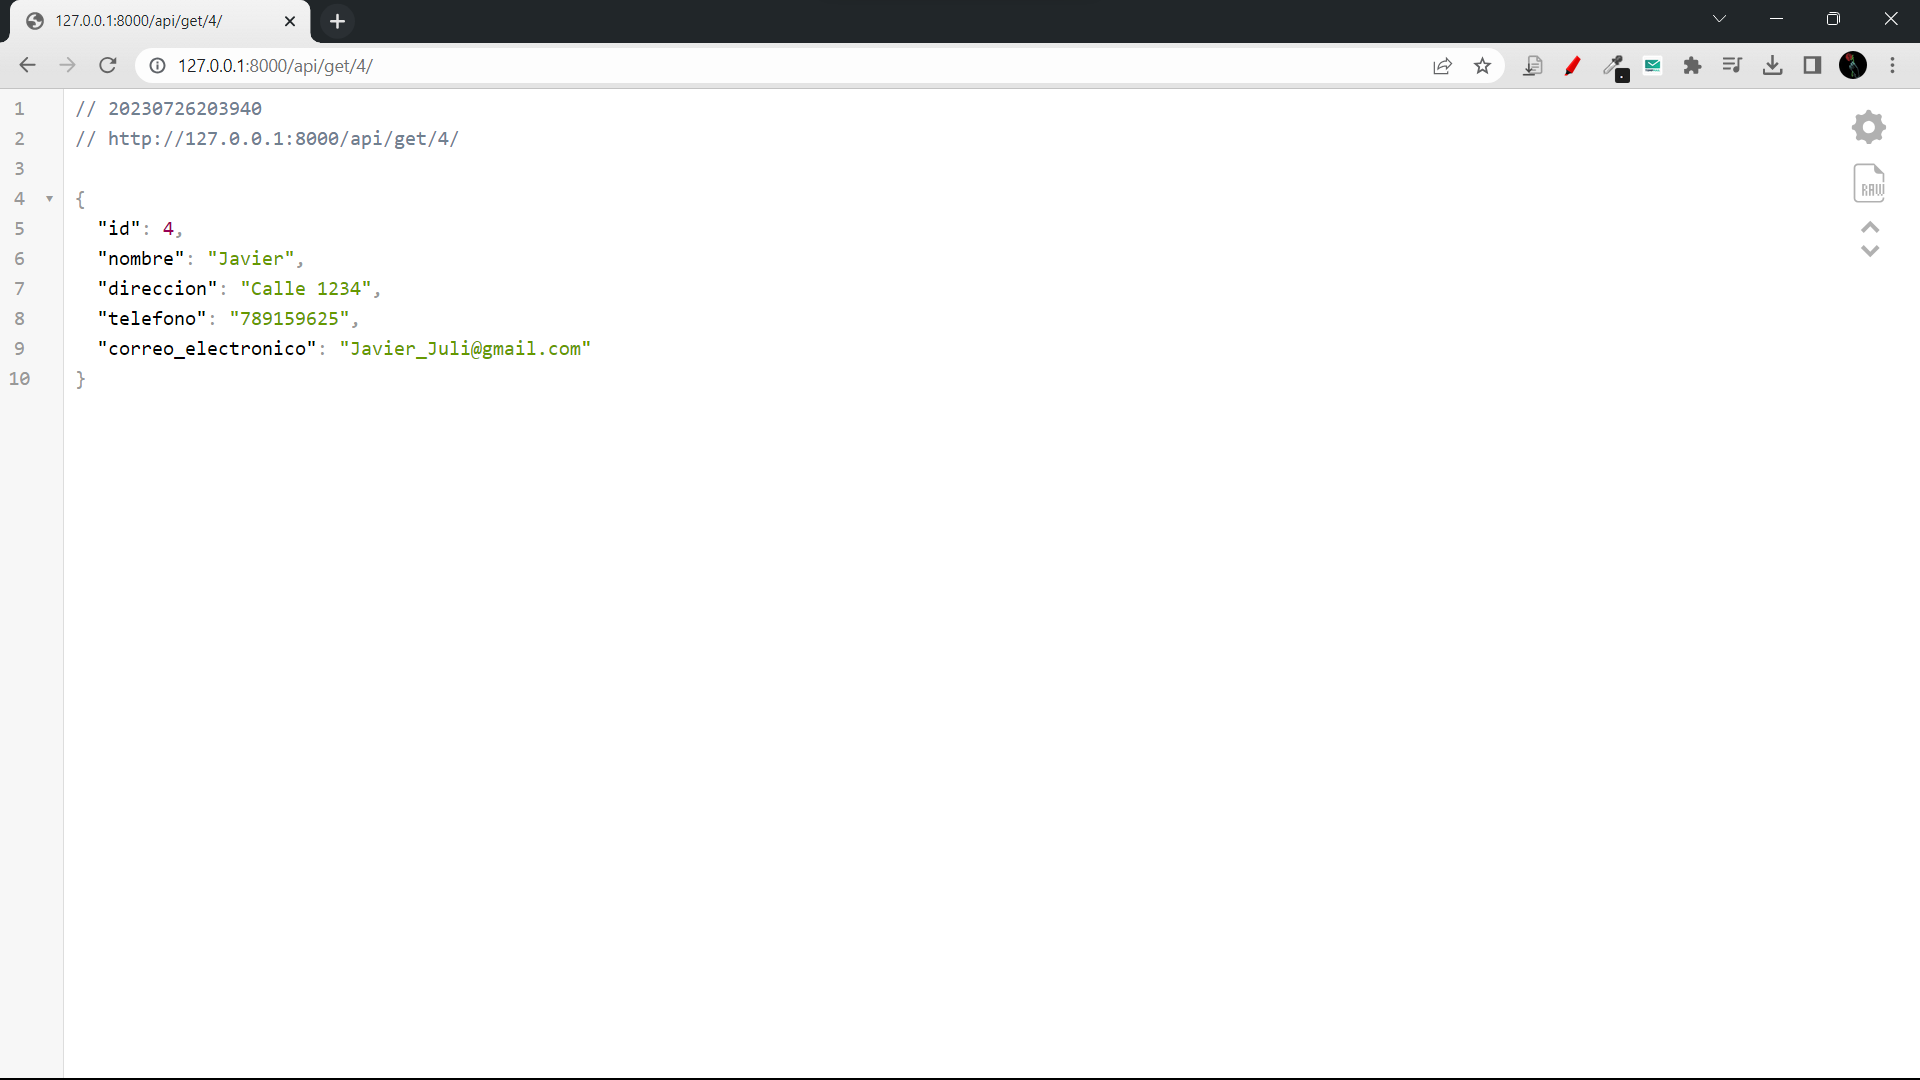
\includegraphics[width=0.9\textwidth,keepaspectratio]{img/DjangoApiRest/getWEB2.png}
            \caption{GET de un contacto desde la web}
            \label{fig:enter-label}
        \end{figure}

    \textbf{POST} - 
    Para el post necesitamos enviar todos los datos en formato JSON dentro del Body, y así optenemos una respuesta correcta y añadimos un nuevo contacto desde nuestra API

        \begin{figure}[H]
            \centering
            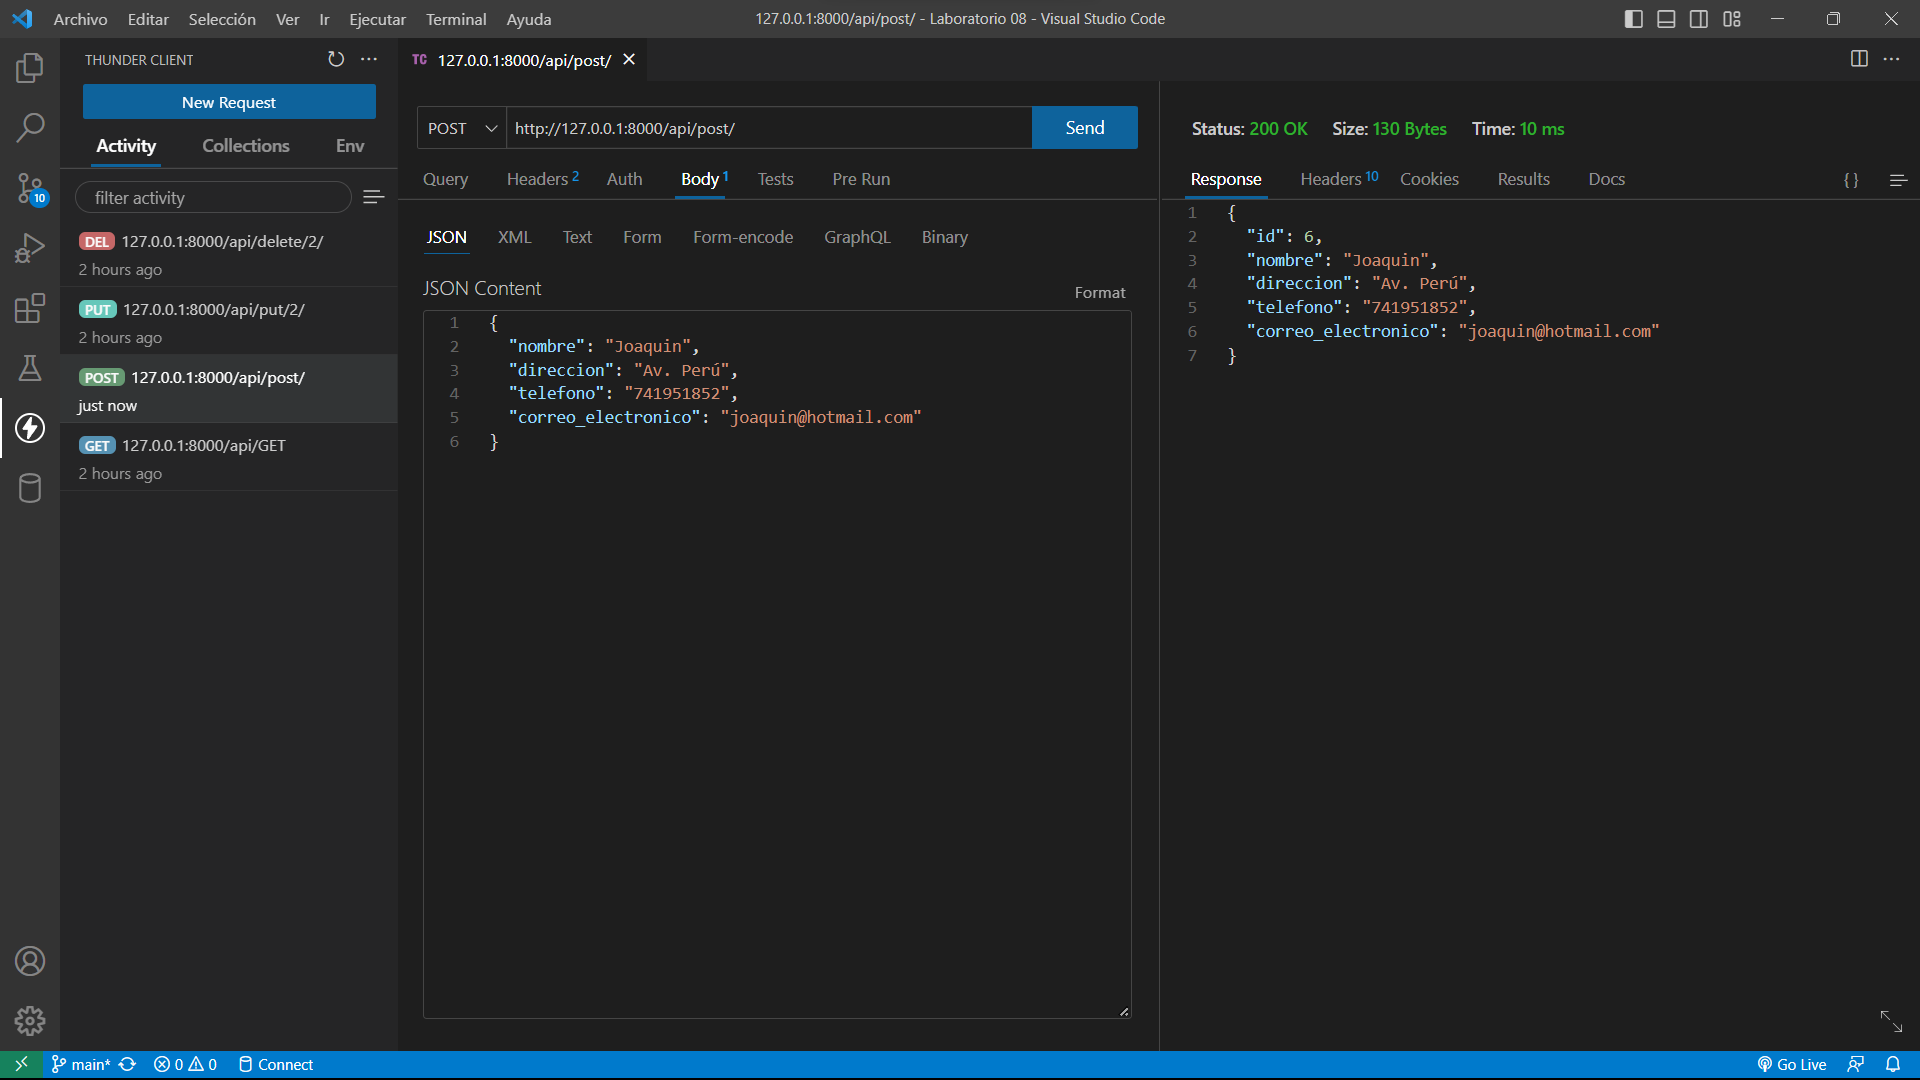
\includegraphics[width=0.9\textwidth,keepaspectratio]{img/DjangoApiRest/post.png}
            \caption{POST de un contacto desde Thunder Client}
            \label{fig:enter-label}
        \end{figure}

    \textbf{PUT} - 
    Para el put, debemos ingresar el id en la url y los demás datos dentro del Body, así hacemos una modificación de todos los datos, de lo contrario, se mandará mensaje de error "Contacto no encontrado"

        \begin{figure}[H]
            \centering
            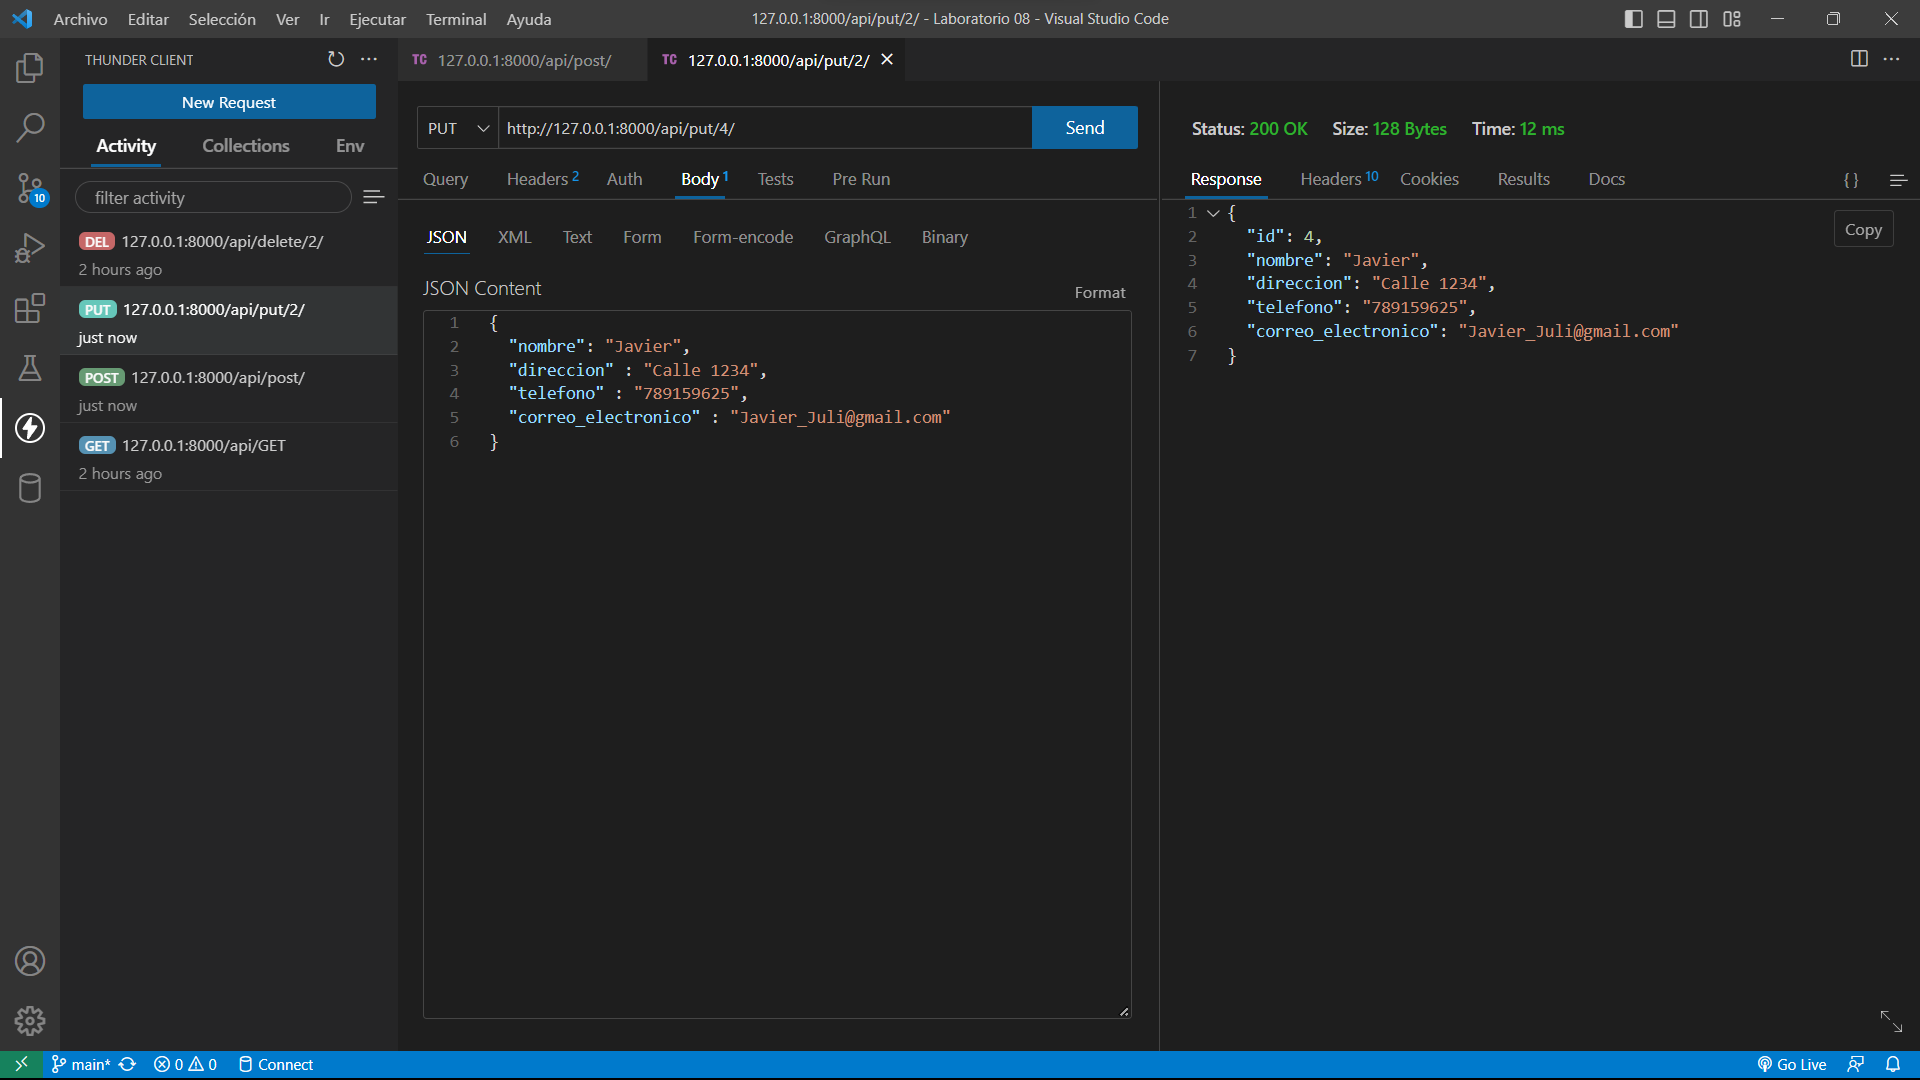
\includegraphics[width=0.9\textwidth,keepaspectratio]{img/DjangoApiRest/put.png}
            \caption{PUT de un contacto desde Thunder Client}
            \label{fig:enter-label}
        \end{figure}
        
    \textbf{DELETE} - 
    Para el delete, debemos de solo ingresar el id del contacto dentro de la url, con esto conseguimos eliminar el contacto deseado, de lo contrario, se mandará mensaje de error "Contacto no encontrado"

        \begin{figure}[H]
            \centering
            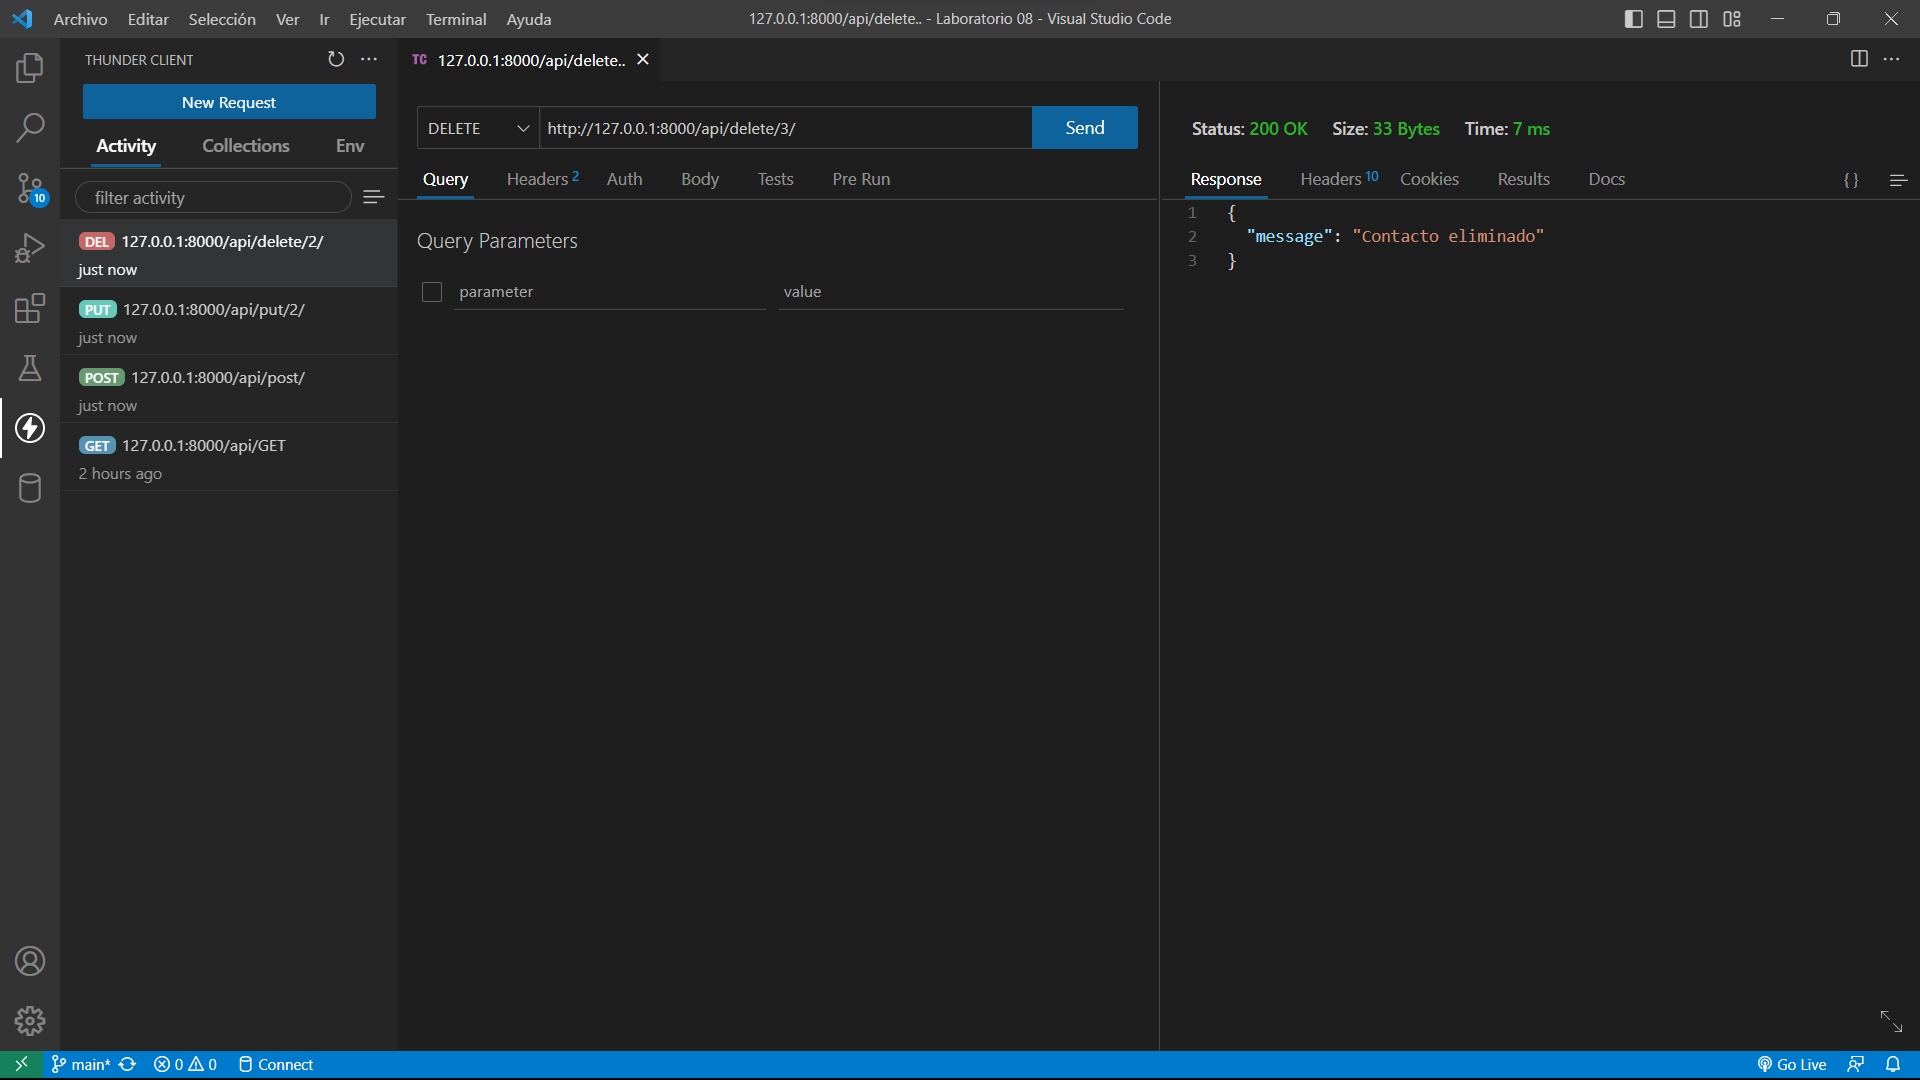
\includegraphics[width=0.9\textwidth,keepaspectratio]{img/DjangoApiRest/delete.png}
            \caption{DELETE de un contacto desde Thunder Client}
            \label{fig:enter-label}
        \end{figure}

    \subsection{Como consumir una API de DNI para Validaciones}
    Como segundo proyecto presentado, es el como consumir una API de la WEB encargada de devolver JSON con información de un DNI, para así validar por ejemplo el registro de cuentas para un Casino Virtual.\\

    Para abrir este servidor debemos ejecutar los siguientes comandos desde nuestra terminal:
    
    \begin{lstlisting}[language=bash,caption={Ingresango a la carpeta dniAPI}][H]
		$ cd dniAPI
	\end{lstlisting}

        Ahora debemos abrir el servidor manage.py
        
        \begin{lstlisting}[language=bash,caption={Abriendo el servidor de este proyecto de consumir API DNI}][H]
		$ python .\manage runserver
	\end{lstlisting}
    
    
    A continuación se presentarán los códigos más importantes de este proyecto con su explicación:\\

    \subsubsection{Proyecto dniAPI}\\

    Primero se definieron las url con las que se trabajará esta simulación de Register y Login de Casino Virtual

    \lstinputlisting[language=Python, caption={dniAPI/urls.py},numbers=left,]{src/dni/urls.py}
    
    \subsubsection{App dni}\\

    Ahora, haremos nuestras modelo para la base de datos, en la que usaremos un modelo y un AUTH personalizado, hecho para nuestra validación:
    
     \lstinputlisting[language=Python, caption={dniAPI/dni/models.py},numbers=left,]{src/dni/models.py}

     Posteriormente, se definieron los forms para el login y register de nuestra aplicación:
    
     \lstinputlisting[language=Python, caption={dniAPI/dni/forms.py},numbers=left,]{src/dni/forms.py}

     Luego, hacemos nuestras views, cada uno con sus validaciones respectivas para lograr una correcta ejecución, mostrando mensaje si la validación no fué exitosa:
    
     \lstinputlisting[language=Python, caption={dniAPI/dni/views.py},numbers=left,]{src/dni/views.py}

    Por ultimo, mostraremos nuestro Home.html dependiendo de si está autenticado o no:
    
     \lstinputlisting[language=HTML, caption={dniAPI/dni/templates/home.html},numbers=left,]{src/dni/home.html}

     \subsubsection{Ejecución}
     Ahora que vimos como funciona nuestro proyecto con el código fuente, podemos proceder a mostrar como es la ejecución

     \textbf{Home sin autenticación}\\\\
     Esto es como se mostrará nuestro Home cuando lo abrimos primera vez, es decir, sin registrarnos:
     
     \begin{figure}[H]
            \centering
            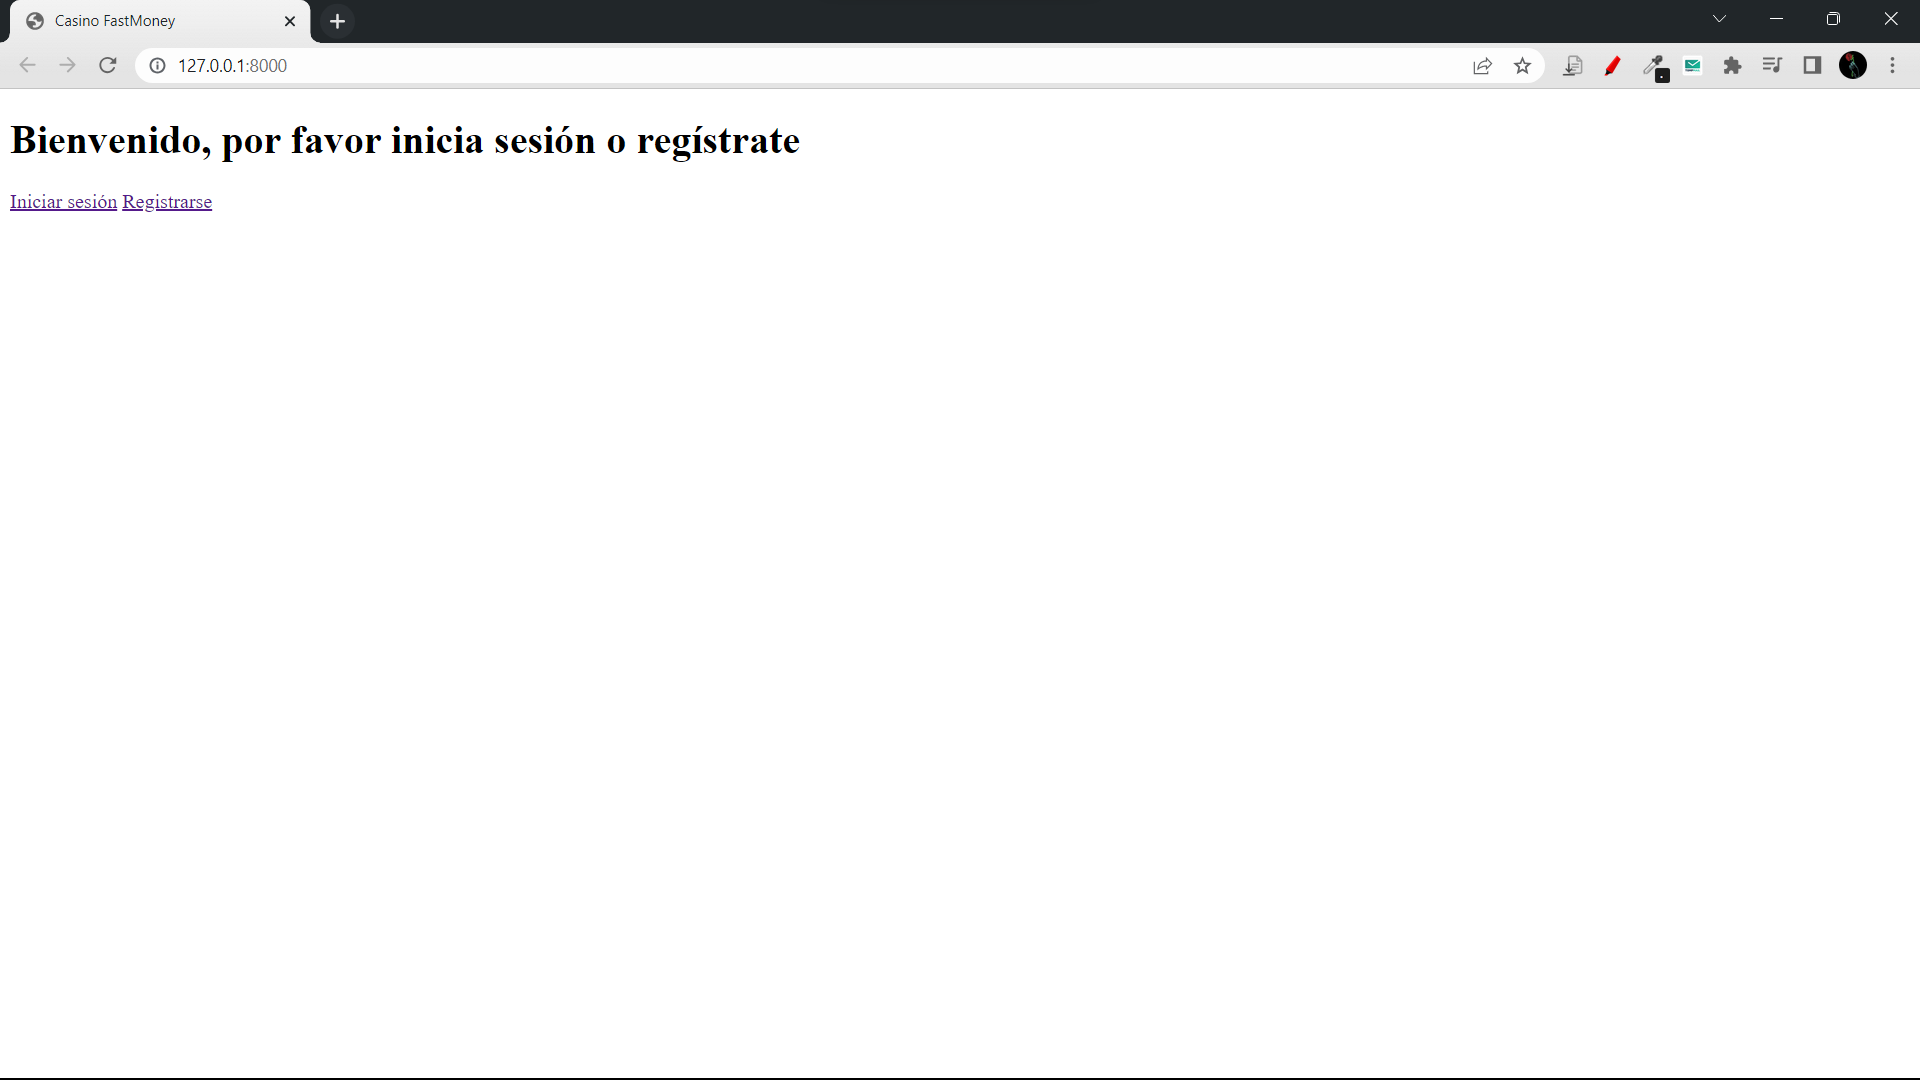
\includegraphics[width=0.9\textwidth,keepaspectratio]{img/dni/homeBasico.png}
            \caption{Home sin autenticarse}
            \label{fig:enter-label}
        \end{figure}

     \textbf{Register inválido}\\\\
     Cuando hay un register invalido mandará un mensaje de alerta, es decir, los datos ingresados, DNI, nombres, apellidos, no coinciden con el dni ingresado, es decir, datos falsos:
     
     \begin{figure}[H]
            \centering
            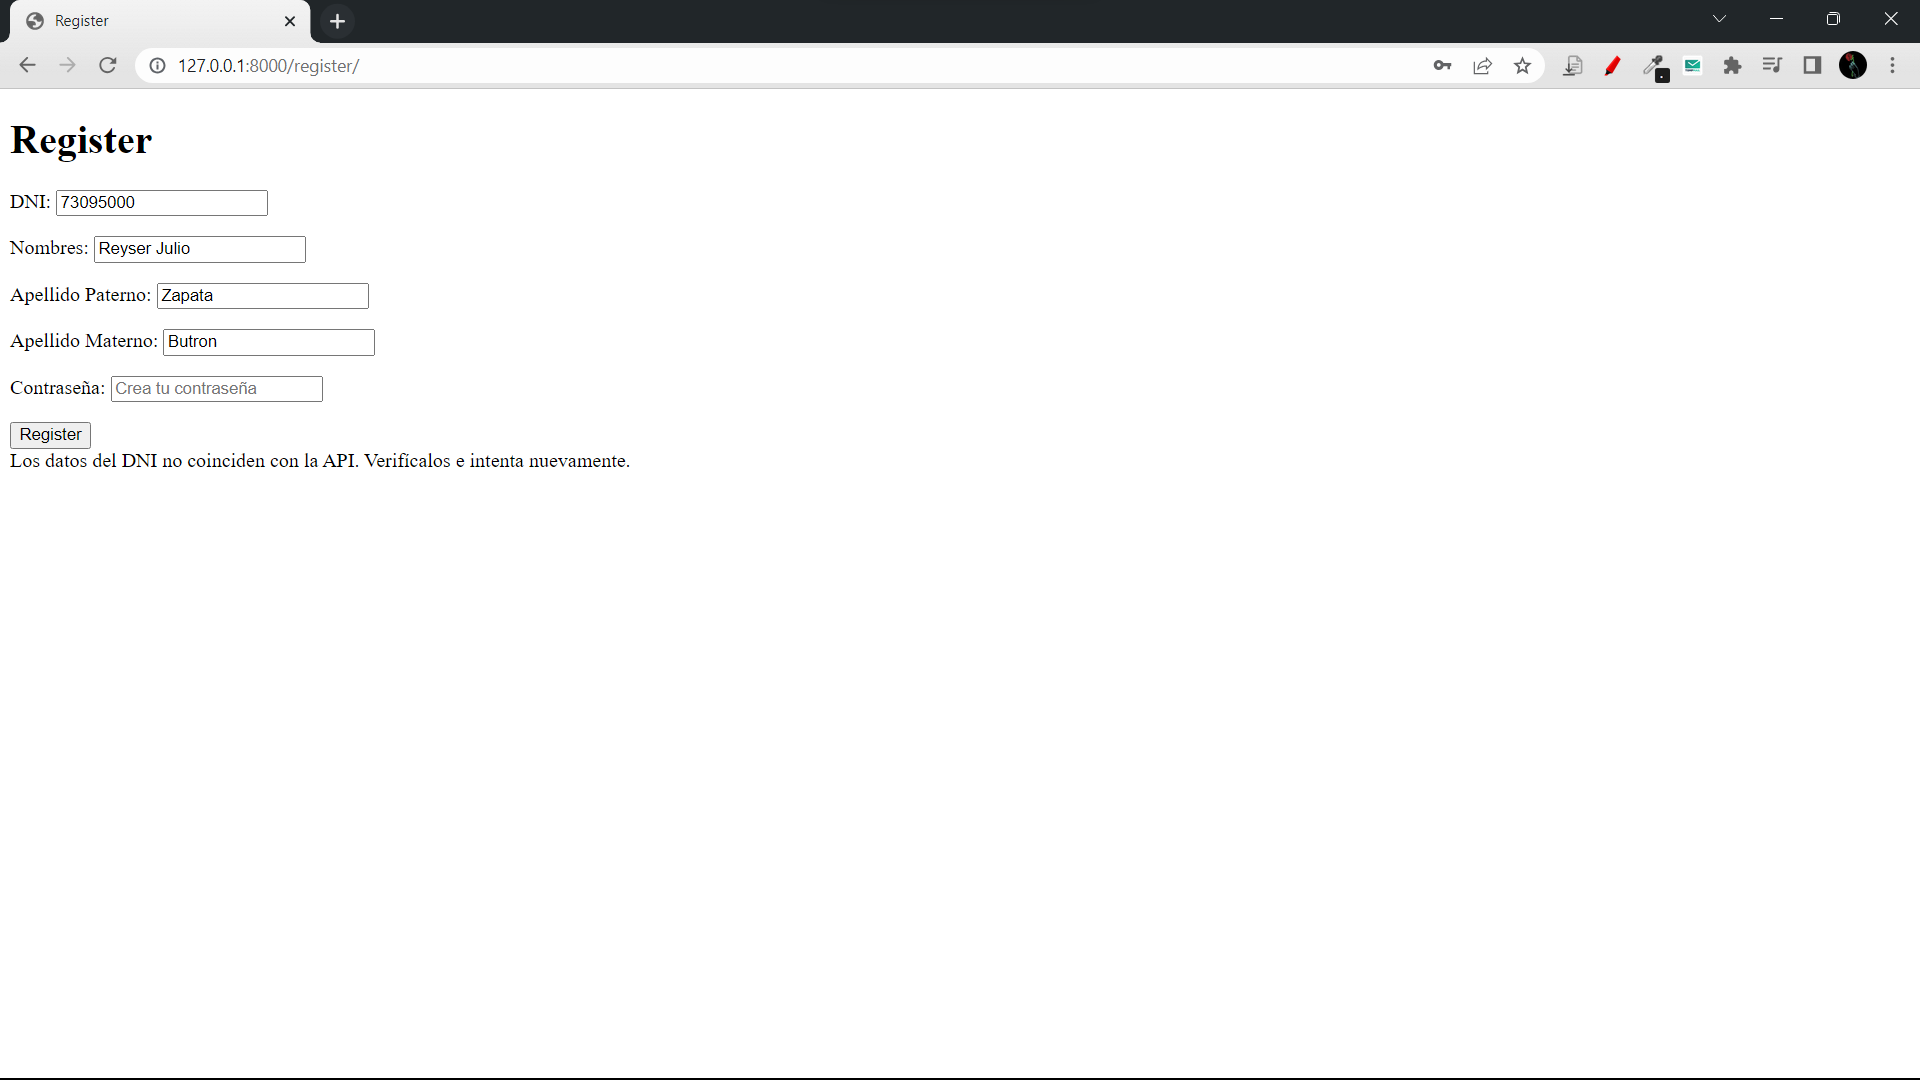
\includegraphics[width=0.9\textwidth,keepaspectratio]{img/dni/registerInvalid.png}
            \caption{Registro inválido}
            \label{fig:enter-label}
        \end{figure}

     \textbf{Register válido}\\\\
        Cuando ingresamos el dni válido, junto con el nombre y apellidos correctos, se nos mandará al Home, para hacer el login correspondiente:
     
        \begin{figure}[H]
            \centering
            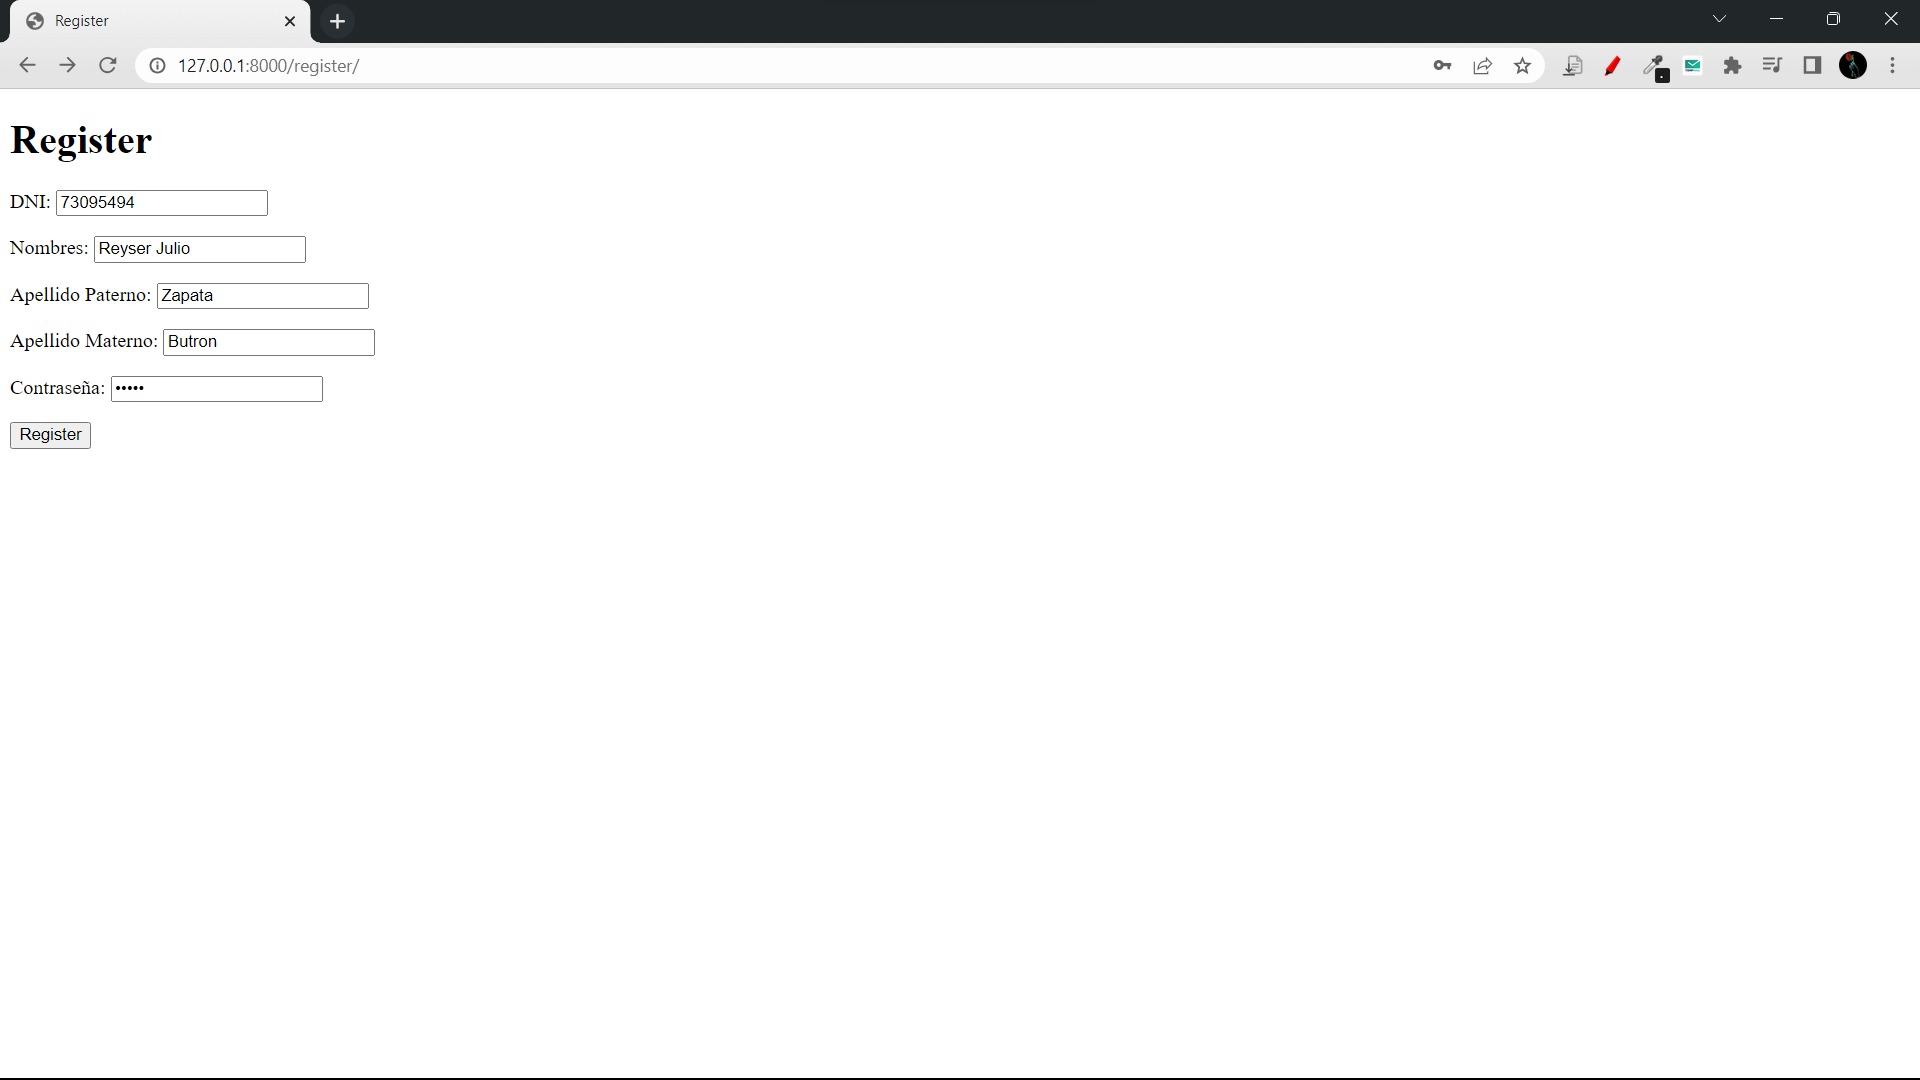
\includegraphics[width=0.9\textwidth,keepaspectratio]{img/dni/registerValid.png}
            \caption{Register con datos válidos}
            \label{fig:enter-label}
        \end{figure}

        Respuesta del Api:
        
        \begin{figure}[H]
            \centering
            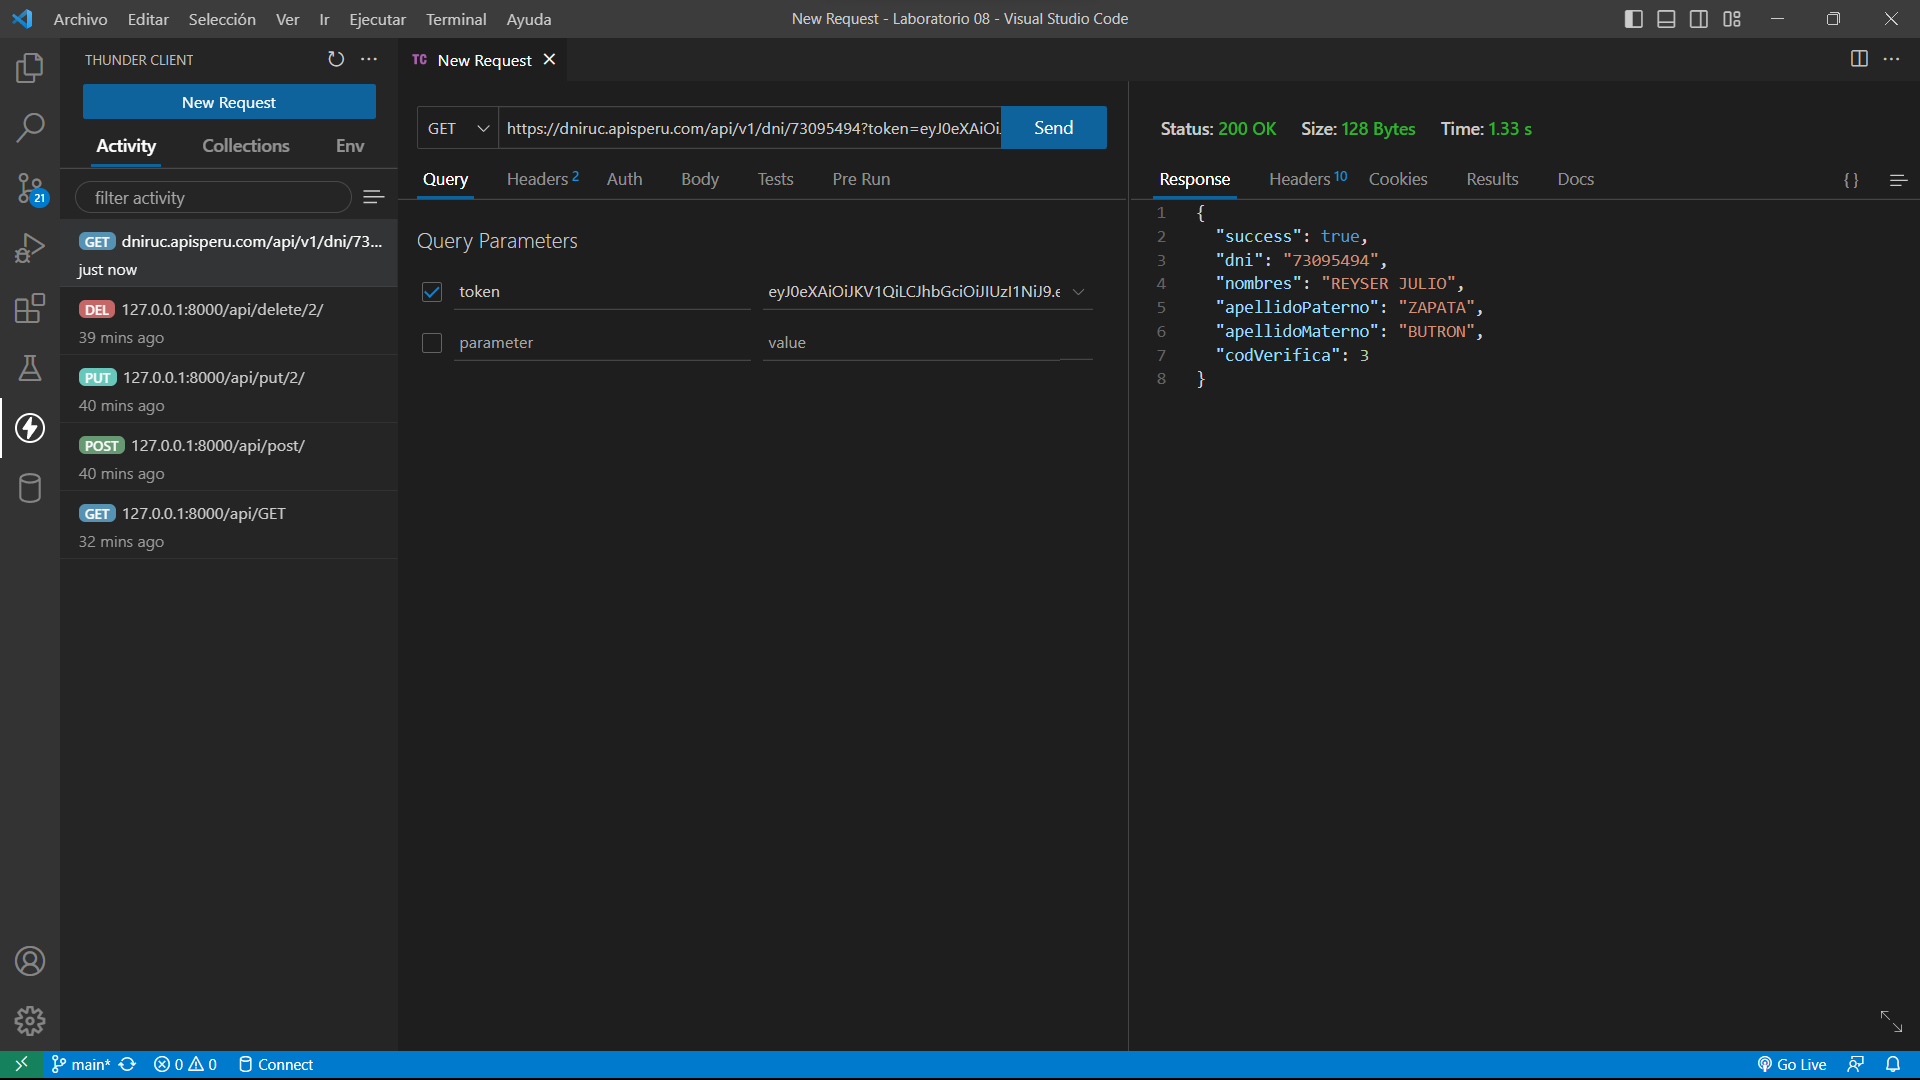
\includegraphics[width=0.9\textwidth,keepaspectratio]{img/dni/apiDNI.png}
            \caption{Respuesta de la API don el dni}
            \label{fig:enter-label}
        \end{figure}

     \textbf{Login}\\\\
        Este es el apartado del Login, es decir, ingresaremos nuestro dni y contraseña:
     
        \begin{figure}[H]
            \centering
            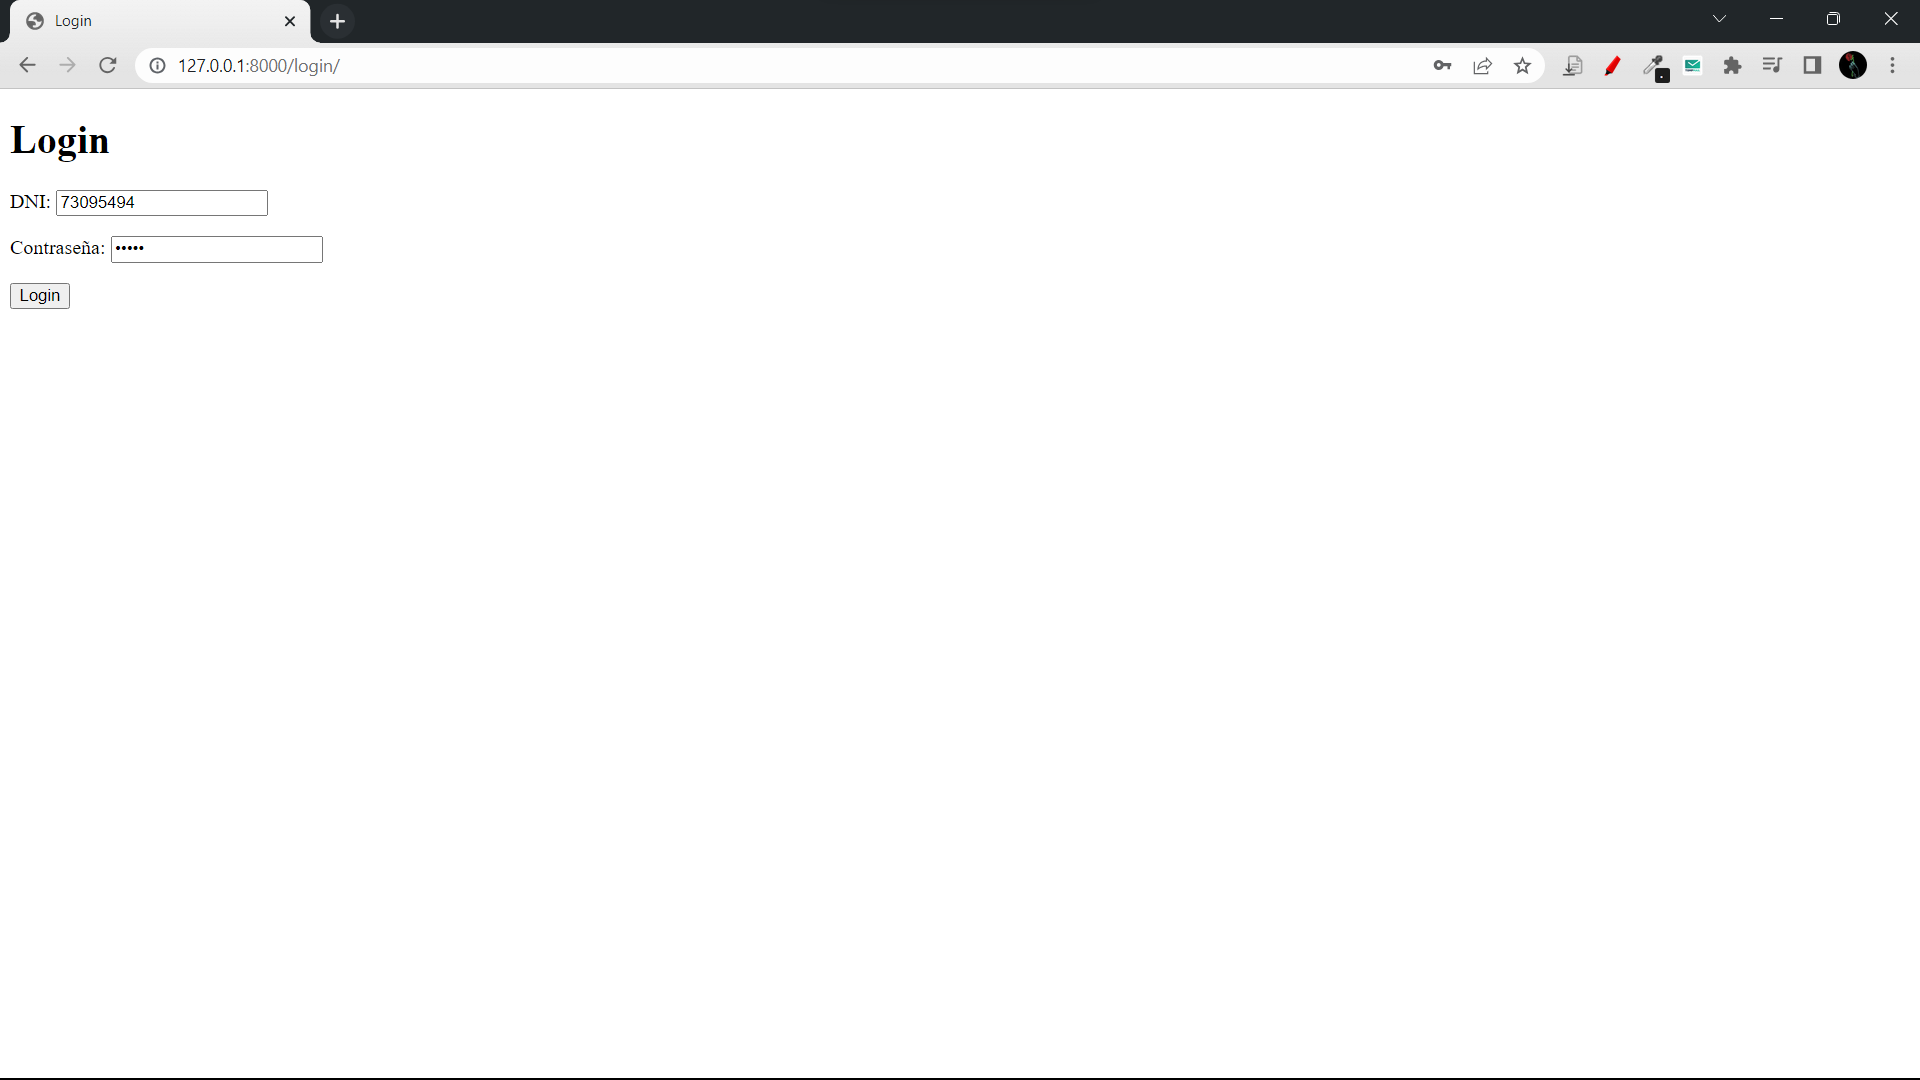
\includegraphics[width=0.9\textwidth,keepaspectratio]{img/dni/login.png}
            \caption{Login.html}
            \label{fig:enter-label}
        \end{figure}

     \textbf{Home autenticado}\\\\
        Cuando hicimos un Login exitoso, el home se nos mostrará de esta forma:
     
        \begin{figure}[H]
            \centering
            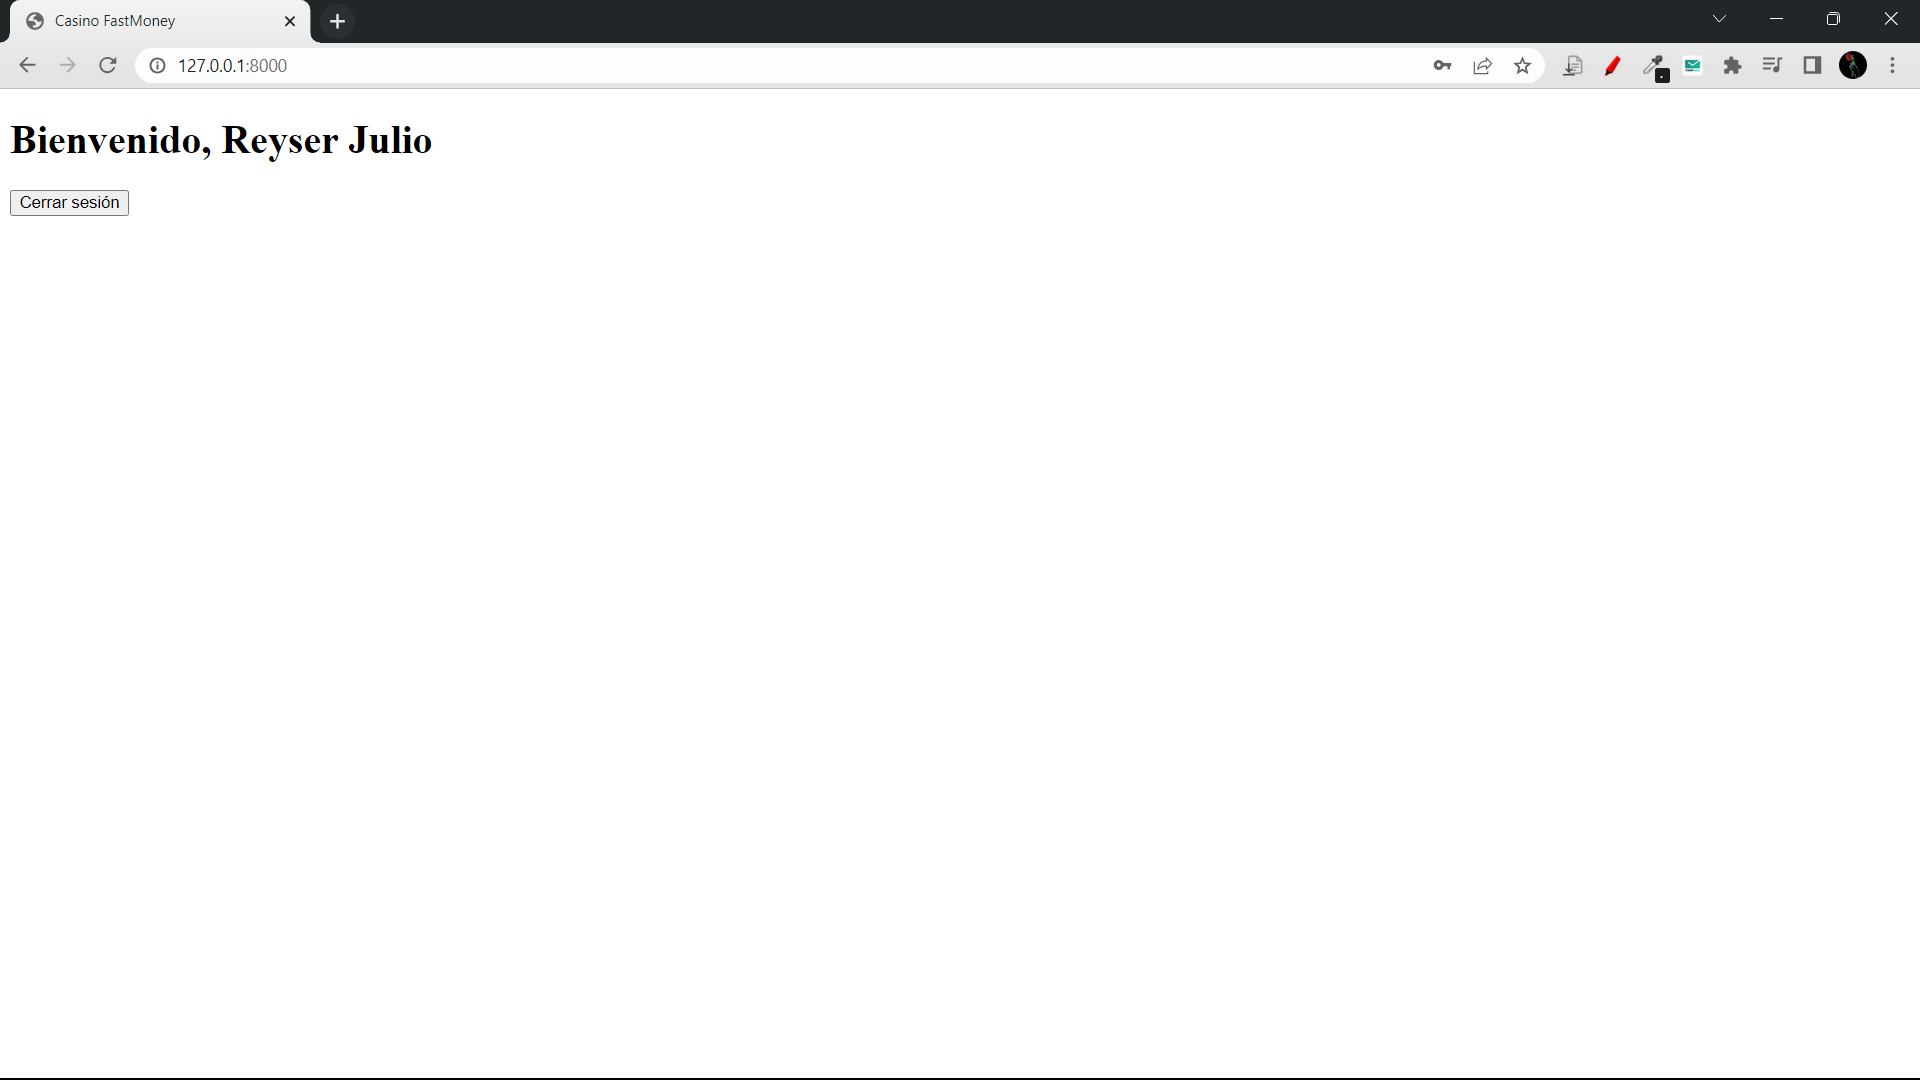
\includegraphics[width=0.9\textwidth,keepaspectratio]{img/dni/homeLogeado.png}
            \caption{Home con login exitoso}
            \label{fig:enter-label}
        \end{figure}
    
\section{Equipos, materiales y temas utilizados}
	\begin{itemize}
		\item Visual Studio 1.80
		\item Python 3.11
		\item Git 2.39.2.
            \item Entorno virtual
		\item Cuenta en GitHub con el correo institucional.
            \item Django 4
		\item Django Rest Framework
	\end{itemize}
	
	\section{URL de Repositorio Github}
	\begin{itemize}
		\item URL del Repositorio GitHub para clonar o recuperar.
		\item \url{https://github.com/ReyserLyn/pweb-lab-08.git}
	\end{itemize}
	
	\section{Actividades con el repositorio GitHub}
	
	\subsection{Clonamos el repositorio GitHub}
	\begin{itemize}	
		\item Al ser un proyecto en repositorio independiente, para su ejecución debemos clonar el repositorio.
	\end{itemize}	
		
	\begin{lstlisting}[language=bash,caption={Clonando Repositorio del Laboratorio 08}][H]
		$ git clone https://github.com/ReyserLyn/pweb-lab-08.git
	\end{lstlisting}
	\begin{lstlisting}[language=bash,caption={Dirijíéndonos al directorio de trabajo}][H]
		$ cd pweb-lab-08
	\end{lstlisting}	

        Una vez estemos dentro de nuestro directorio de trabajo, tenemos que crear el entorno virtual, activarlo e instalar las dependencias necesarias para la correcta ejecución de los proyectos.
        
	\begin{lstlisting}[language=bash,caption={Creando entorno virtual}][H]
		$ py -m venv venv
	\end{lstlisting}
         \begin{lstlisting}[language=bash,caption={Activamos nuestro entorno virtual}][H]
		$ venv/Scripts/activate
	\end{lstlisting}
	\begin{lstlisting}[language=bash,caption={Descargando dependencias}][H]
		$ pip install -r requirements.txt
	\end{lstlisting}

        Una vez tengamos esto hecho, ya podremos abrir los servidor de los diferentes proyectos y probar su funcionalidad.
	
	\subsection{Estructura de laboratorio 08}
	\begin{itemize}	
		\item El contenido que se entrega en este laboratorio es el siguiente:
	\end{itemize}
	
\begin{lstlisting}[style=ascii-tree]
pweb-lab-08/
|--- djaangoApiRest
    |--- api
        |--- migrations
        |--- __init__.py
        |--- admin.py
        |--- apps.py
        |--- models.py
        |--- serializers.py
        |--- tests.py
        |--- urls.py
        |--- views.py
    |--- asgi.py
    |--- middleware.py
    |--- settings.py
    |--- urls.py
    |--- wsgi.py
|--- dniAPI
    |--- dni
        |--- migrations
        |--- static
        |--- templates
        |--- __init__.py
        |--- admin.py
        |--- apps.py
        |--- forms.py
        |--- models.py
        |--- tests.py
        |--- views.py
    |--- __init__.py
    |--- asgi.py
    |--- db.sqlite3
    |--- manage.py
    |--- settings.py
    |--- urls.py
    |--- wsgi.py
|--- Latex (Informe Latex)
|--- Tutorial (Ejercicio Django - QuickStart)
|--- .gitignore
|--- db
|--- manage.py
|--- requirements.txt

\end{lstlisting}    

Siendo el directorio más importante "DjangoApiRest", es donde se evidencia nuestra CRUD API.

\subsection{Commits}
    En la captura de pantalla mostrada a continuación, se pueden ver los commits más importantes tratados para este Laboratorio 08:
    
       \begin{figure}[H]
            \centering
            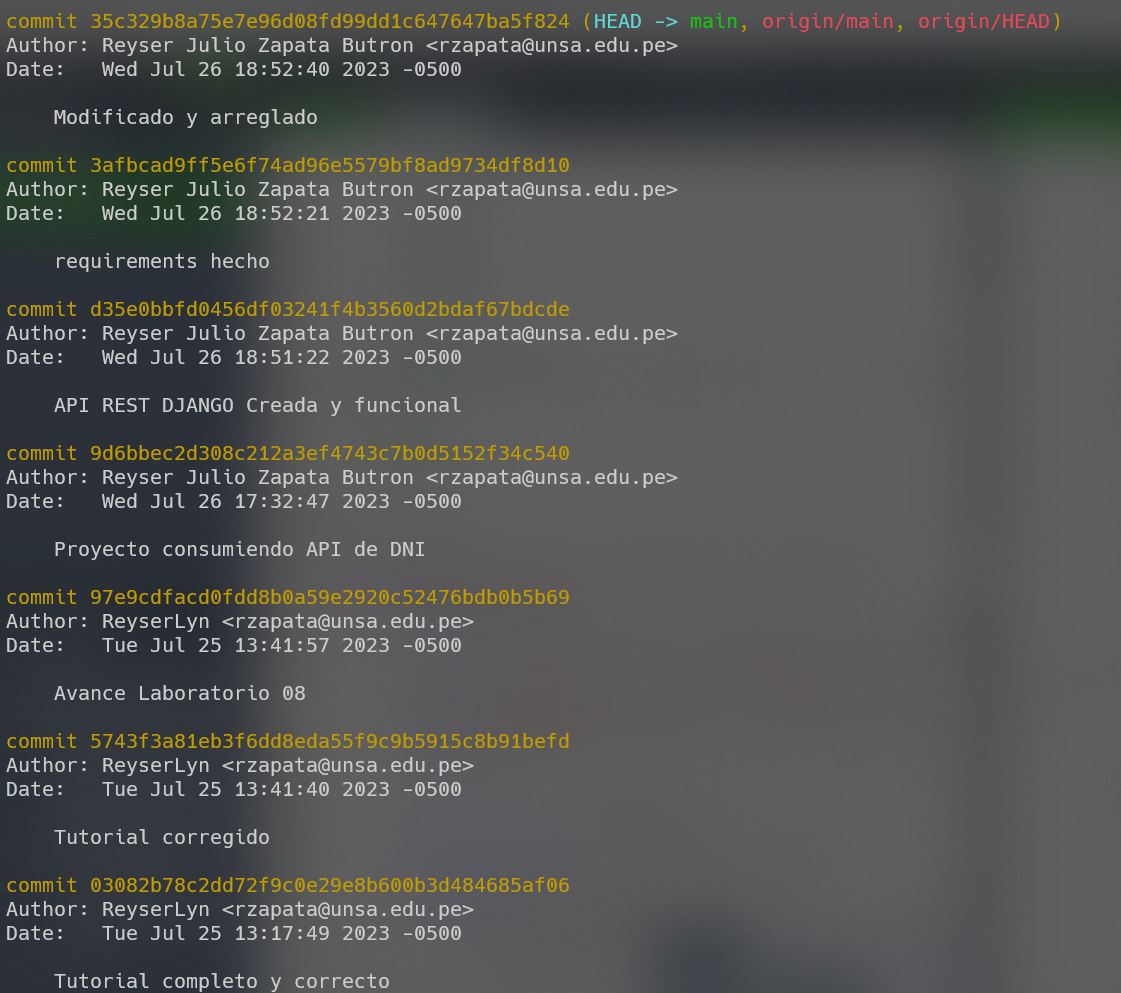
\includegraphics[width=0.9\textwidth,keepaspectratio]{img/commits.png}
            \caption{Captura de pantalla de los commits más importantes}
            \label{fig:enter-label}
        \end{figure}

\section{Pregunta: ¿Cúal fué la mayor dificultad del uso de este framework?}
La mayor dificultad que enfrentamos al usar este framework fue familiarizarnos con su estructura y conceptos clave. Al principio, nos resultó un poco abrumador entender cómo se organiza el proyecto, cómo definir modelos, serializadores y vistas, y cómo configurar las rutas para las API. Sin embargo, a medida que avanzamos en el desarrollo y consultamos la documentación oficial y otros recursos, pudimos superar esta dificultad y comprender mejor cómo aprovechar todas las capacidades que ofrece Django Rest Framework. Una vez superado este obstáculo inicial, pudimos aprovechar al máximo las funcionalidades del framework y desarrollar una API robusta y eficiente para nuestro proyecto.

\section{\textcolor{red}{Rúbricas}}
	
	\subsection{\textcolor{red}{Entregable Informe}}
	\begin{table}[H]
		\caption{Tipo de Informe}
		\setlength{\tabcolsep}{0.5em} % for the horizontal padding
		{\renewcommand{\arraystretch}{1.5}% for the vertical padding
		\begin{tabular}{|p{3cm}|p{12cm}|}
			\hline
			\multicolumn{2}{|c|}{\textbf{\textcolor{red}{Informe}}}  \\
			\hline 
			\textbf{\textcolor{red}{Latex}} & \textcolor{blue}{El informe está en formato PDF desde Latex,  con un formato limpio (buena presentación) y facil de leer.}   \\ 
			\hline 
		\end{tabular}
	}
	\end{table}
	
	\clearpage
	
	\subsection{\textcolor{red}{Rúbrica para el contenido del Informe y demostración}}
	\begin{itemize}			
		\item El alumno debe marcar o dejar en blanco en celdas de la columna \textbf{Checklist} si cumplio con el ítem correspondiente.
		\item Si un alumno supera la fecha de entrega,  su calificación será sobre la nota mínima aprobada, siempre y cuando cumpla con todos lo items.
		\item El alumno debe autocalificarse en la columna \textbf{Estudiante} de acuerdo a la siguiente tabla:
	
		\begin{table}[ht]
			\caption{Niveles de desempeño}
			\begin{center}
			\begin{tabular}{ccccc}
    			\hline
    			 & \multicolumn{4}{c}{Nivel}\\
    			\cline{1-5}
    			\textbf{Puntos} & Insatisfactorio 25\%& En Proceso 50\% & Satisfactorio 75\% & Sobresaliente 100\%\\
    			\textbf{2.0}&0.5&1.0&1.5&2.0\\
    			\textbf{4.0}&1.0&2.0&3.0&4.0\\
    		\hline
			\end{tabular}
		\end{center}
	\end{table}	
	
	\end{itemize}
	
	\begin{table}[H]
		\caption{Rúbrica para contenido del Informe y demostración}
		\setlength{\tabcolsep}{0.5em} % for the horizontal padding
		{\renewcommand{\arraystretch}{1.5}% for the vertical padding
		%\begin{center}
		\begin{tabular}{|p{2.7cm}|p{7cm}|x{1.3cm}|p{1.2cm}|p{1.5cm}|p{1.1cm}|}
			\hline
    		\multicolumn{2}{|c|}{Contenido y demostración} & Puntos & Checklist & Estudiante & Profesor\\
			\hline
			\textbf{1. GitHub} & Hay enlace URL activo del directorio para el  laboratorio hacia su repositorio GitHub con código fuente terminado y fácil de revisar. &2 &X &2 & \\ 
			\hline
			\textbf{2. Commits} &  Hay capturas de pantalla de los commits más importantes con sus explicaciones detalladas. (El profesor puede preguntar para refrendar calificación). &4 &X &4 & \\ 
			\hline 
			\textbf{3. Código fuente} &  Hay porciones de código fuente importantes con numeración y explicaciones detalladas de sus funciones. &2 &X &2 & \\ 
			\hline 
			\textbf{4. Ejecución} & Se incluyen ejecuciones/pruebas del código fuente  explicadas gradualmente. &2 &X &2 & \\ 
			\hline			
			\textbf{5. Pregunta} & Se responde con completitud a la pregunta formulada en la tarea.  (El profesor puede preguntar para refrendar calificación).  &2 &X &2 & \\ 
			\hline	
			\textbf{6. Fechas} & Las fechas de modificación del código fuente estan dentro de los plazos de fecha de entrega establecidos. &2 & &0 & \\ 
			\hline 
			\textbf{7. Ortografía} & El documento no muestra errores ortográficos. &2 &X &2 & \\ 
			\hline 
			\textbf{8. Madurez} & El Informe muestra de manera general una evolución de la madurez del código fuente,  explicaciones puntuales pero precisas y un acabado impecable.   (El profesor puede preguntar para refrendar calificación).  &4 &X &4 & \\ 
			\hline
			\multicolumn{2}{|c|}{\textbf{Total}} &20 & &18 & \\ 
			\hline
		\end{tabular}
		%\end{center}
		%\label{tab:multicol}
		}
	\end{table}
	
\clearpage

\section{Referencias}
\begin{itemize}			
	\item \url{https://www.django-rest-framework.org/tutorial/quickstart/}
	\item \url{https://www.django-rest-framework.org/tutorial/4-authentication-and-permissions/}
 \item \url{https://coffeebytes.dev/como-personalizar-el-modelo-user-en-django/}
 \item \url{https://www.django-rest-framework.org/}
\end{itemize}	
\end{document}